% Options for packages loaded elsewhere
\PassOptionsToPackage{unicode}{hyperref}
\PassOptionsToPackage{hyphens}{url}
%
\documentclass[
]{article}
\usepackage{amsmath,amssymb}
\usepackage{lmodern}
\usepackage{ifxetex,ifluatex}
\ifnum 0\ifxetex 1\fi\ifluatex 1\fi=0 % if pdftex
  \usepackage[T1]{fontenc}
  \usepackage[utf8]{inputenc}
  \usepackage{textcomp} % provide euro and other symbols
\else % if luatex or xetex
  \usepackage{unicode-math}
  \defaultfontfeatures{Scale=MatchLowercase}
  \defaultfontfeatures[\rmfamily]{Ligatures=TeX,Scale=1}
\fi
% Use upquote if available, for straight quotes in verbatim environments
\IfFileExists{upquote.sty}{\usepackage{upquote}}{}
\IfFileExists{microtype.sty}{% use microtype if available
  \usepackage[]{microtype}
  \UseMicrotypeSet[protrusion]{basicmath} % disable protrusion for tt fonts
}{}
\makeatletter
\@ifundefined{KOMAClassName}{% if non-KOMA class
  \IfFileExists{parskip.sty}{%
    \usepackage{parskip}
  }{% else
    \setlength{\parindent}{0pt}
    \setlength{\parskip}{6pt plus 2pt minus 1pt}}
}{% if KOMA class
  \KOMAoptions{parskip=half}}
\makeatother
\usepackage{xcolor}
\IfFileExists{xurl.sty}{\usepackage{xurl}}{} % add URL line breaks if available
\IfFileExists{bookmark.sty}{\usepackage{bookmark}}{\usepackage{hyperref}}
\hypersetup{
  pdftitle={Relocation choice for different homophily preferences: hybrid scenarios for Schelling Model},
  pdfkeywords={super-diversity, discrete choice, spatial sorting,
Schelling},
  hidelinks,
  pdfcreator={LaTeX via pandoc}}
\urlstyle{same} % disable monospaced font for URLs
\usepackage[margin=1in]{geometry}
\usepackage{graphicx}
\makeatletter
\def\maxwidth{\ifdim\Gin@nat@width>\linewidth\linewidth\else\Gin@nat@width\fi}
\def\maxheight{\ifdim\Gin@nat@height>\textheight\textheight\else\Gin@nat@height\fi}
\makeatother
% Scale images if necessary, so that they will not overflow the page
% margins by default, and it is still possible to overwrite the defaults
% using explicit options in \includegraphics[width, height, ...]{}
\setkeys{Gin}{width=\maxwidth,height=\maxheight,keepaspectratio}
% Set default figure placement to htbp
\makeatletter
\def\fps@figure{htbp}
\makeatother
\setlength{\emergencystretch}{3em} % prevent overfull lines
\providecommand{\tightlist}{%
  \setlength{\itemsep}{0pt}\setlength{\parskip}{0pt}}
\setcounter{secnumdepth}{-\maxdimen} % remove section numbering
\usepackage{float}
\usepackage{multirow}
\usepackage{subcaption}
\usepackage[round]{natbib}
\usepackage{xfrac}
\usepackage{booktabs}
\usepackage{longtable}
\usepackage{array}
\usepackage{multirow}
\usepackage{wrapfig}
\usepackage{float}
\usepackage{colortbl}
\usepackage{pdflscape}
\usepackage{tabu}
\usepackage{threeparttable}
\usepackage{threeparttablex}
\usepackage[normalem]{ulem}
\usepackage{makecell}
\usepackage{xcolor}
\ifluatex
  \usepackage{selnolig}  % disable illegal ligatures
\fi
\usepackage[]{natbib}
\bibliographystyle{apalike}

\title{Relocation choice for different homophily preferences: hybrid
scenarios for Schelling Model}
\author{Rocco Paolillo\\
Andreas Flache\\
~\\
\textbf{\texttt{HERE\ SOME\ NOTES\ TO\ BEAR\ IN\ MIND}}~\\
\textbf{\texttt{Next\ coming:\ figures\ from\ secondary\ beta\ proportional\ to\ dominant\ preference}}~\\
\textbf{\texttt{}}~\\
\textbf{\texttt{}}~\\}
\date{30/09/21 10:15}

\begin{document}
\maketitle

\newcommand{\rocco}[1]{{\textcolor{red}{Rocco: #1}}}

\newcommand{\andreas}[1]{\textcolor{blue}{{Andreas: }#1}}

\abstract{{\textcolor{red}{Rocco: 200 words, 3-5 keywords}} Schelling model of residential segregation famously showed how high levels of residential segregation can emerge as unintended outcome of the interplay of individual relocations of actors who hold relatively mild ethnic preferences.
Most of the work building on this model neglected two forms of heterogeneity which seem to become increasingly important empirically in contemporary societies. 
First, there is considerable heterogeneity of residential preferences not only between but also within ethnic groups, with especially younger, higher educated and more wealthy individuals having less strong preferences for ethnic homophily.
Second, most of the research following Schelling focuses on ethnic similarity as relevant to residential preferences. However, recent theoretical and empirical research on spatial sorting emphasizes multidimensionality, as individuals prefer similar others not only regarding ethnicity, but also for social distinctions as shared values or shared status. Extending recent work (Paolillo et Lorenz, 2018), we explore the interplay of heterogeneity in both forms of homophily preferences for ethnicity and shared values.
Using a discrete choice version of Schelling model, in which agents differ in their relative weights for ethnic and value similarity in relocation moves, we explore the consequences of different preferences of agents and their strengths, in addition to structural conditions of relative group sizes of ethnic and value groups. We find in particular that hybrid segregation patterns can emerge in which ethnically mixed but value homogeneous neighborhoods arise alongside ethnically segregated neighborhoods populated by agents driven more by ethnic homophily. 
Importantly and contrary to Schelling’s model, we show how partial ethnic mixing can arise even if everyone has a preference for more co-ethnics in her neighborhood, all other things being equal.}

\hypertarget{introduction}{%
\section{Introduction}\label{introduction}}

Diversity is an undeniable trait of many modern Western societies. Even though ethnic segregation is decreased over the years, this is still a critical topic and it interacts with new forms of segregations, e.g. segregation by socio-demographich characteristics, as income, religion or else. Schelling \cite{schelling1969models,schelling1971dynamic} demonstrated with a formal computational model how segregation can be a self-organizing phenomenon emerging as an outcome of relocation of agents driven by "discriminatory individual choice" \citep[p. 488]{schelling1969models}. Still today, much modeling literature draws on the essential concept of Schelling model of "preference dynamics" \citep{clark2008understanding} and homophily behavior. Most recent models, however, have extended characteristics of the Schelling model  to reflect the complexity of segregation scenarios in diverse cities, such as change in the shape of utility as preference for ethnic diversity \cite{zhang2004,zhang2011}, mixed preferences for segregation and integration \cite{hatna2012schelling}, or strenght of preferences in relocation choice \cite{bruch2006neighborhood,bruch2009preferences}. However, in this paper we build on different aspects neglected by these models to extend Schelling model to show more hybrid segregation scenarios. First, we build on empirical literature that shows how different socio-demographic characteristics can be associated for different homophilic preferences over different dimensions. We build our model extending Schelling model to random utility model for a combination of ethnic and secondary cross-ethnic preferences. In a formal model, we define value preference as homophily behavior based on cross-ethnic characteristics, and investigate the effect of strenght for either or a combination of both preferences in Schelling-type dynamics.
We propose some mechanisms of hybrid segregation scenarios we observe, showing how partial integration can emerge despite high preference for ethnic similarity. We found that a by-product value segregation of conservative agents who not care for value similarity. The mechanism is modulated by....

\hypertarget{Theory Section}{%
\section{Theory Section}\label{theorysection}}

\subsection{Urban Diversity in modern societies, a fit for Schelling Model?}

Schelling wrote a couple of influential papers demonstrating how spatial segregation can occur as an emergent outcome out of relocation of people within spatial constraints, and how also weak preferences (not being in the minority) could generate segregation.
Though he elaborated a formal model not aimed at being representative of a specific context, he stressed out his attention was towards black and white, in a period when discriminatory housing policies in U.S. were abolished, in a context of white majority and black minority. The aim of the model was to demonstrate how segregation could persist even in case of mild preferences, the main argument was the distinction to be twofold, exhaustive and mutual exclusive.
Schelling model had a legacy in much literature on spatial segregation in the next years, also in empirical literature outside of the computational modelling literature. Schelling model would have been taken as a model based on ethnic preferences where only one dimension was considered, often in a context of majority/minority condition. However, recent trends both in academic literature and empirical census, challenge this context often applied to spatial segregation and Schelling model. In particular, the paradigm of superdiversity has emerged as an alternative to a majority/minority and one-dimensional paradigm of societal and urban landscape \citep{vertovec2007super}. The paradigm stresses the diversity of modern societies as an aggregative effect of migration flows processes of integration through generations in receiving society. Two aspects of superdiversity are important for urban diversity and Schelling-type dynamics. First, the "diversification of diversity" stresses how multiple dimension of diversity exist in addition to ethnic membership, e.g. income, culture, education, etc. Second, how the majority/minorty paradigm is challenged by an amalgama of many ethnic minorities.

Recent residential segreation studies show how diversity is a keen element of urban diversity, and a more complex picture of conclusions from Schelling model. Ethnic segregation in the U.S. has reduced since the 60's/70's \citep{glaeser2012end}, along with reduced racial prejudice (goldman), with an actual increase of ethnically mixed neighborhoods in multi-diverse cities \citep{clark2015residential}. Reasons for this is a structural diversity in the composition of population \citep{lee2012racial}, \citet{crul2016super} shows how in some neighborhoods of multi-diverse cities, second and further generation migrants outnumber native population. However, differences still persist when looking at specific substrata of the population. For instance, lower incomes minorities are more likely to live in both ethnically and socio-economic segregated neighborhoods, with younger generations in more affluent neighborhoods. 
Residential preferences can vary based on socio-demographic characteristics. On the whole, younger \citep{clark2009changing,clark2018can}, more highly educated and higher income citizeens have more tolerant ethnic preferences when it comes to neighborhood choice \citep{clark2009changing,clark2019neighborhood,crowder2012neighborhood}. A recent trend in spatial segregation research has investigated how residential preferences can be affected by socio-cultural disposition \citep{van2019sociocultural} or  political homophily. These are an example of value homophily preferences.

\subsection{Schelling literature for complex scenarios}

Hatna and Benson, Xie e zhou

\subsection{Discrete choice models}
Bruch etc. why we want to extend to discrete choice

\subsection{Final statement and contribution of the paper}

\hfill \newline

Ethnic or racial residential segregation appears still a critical topic
of multi-ethnic cities all over the world \citep{charles2003dynamics}.
Many possible and interconnected explanations for segregation have been
proposed, such as discrimination by landlords
\citep{ahmed2008discrimination}, the sorting mechanisms built into
housing markets \citep{bailey2012spatial}, or income inequality in
combination with features of urban geography
\citep{pais2017intergenerational}. Prominently,
\cite{schelling1969models,schelling1971dynamic}'s contribution was to
demonstrate with a formal computational model that segregation can be a
self-organizing phenomenon that emerges from the interaction of people
satisfying their ``discriminatory individual choice''
\citep[p. 488]{schelling1969models} within spatial limited
constraints\footnote{Essentially the same mechanism proposed by Schelling was independently developed and formalized earlier by \cite{sakoda1971checkerboard}, see \cite{hegselmann2017thomas}}.
Essential to Schelling's model, and focus of this paper, is the concept
of ``preference dynamics'' \citep{clark2008understanding}, i.e.~the
empirically plausible assumption that people typically want at least a
certain minimal fraction of co-ethnics nearby, even if they are content
with living in a mixed neighborhood. One key insight from a large number
of formal modelling studies is the robustness of the main results of the
model \citep{flache2020analytical}, also if people hold
``integrationist'' preferences \citep{zhang2004} or randomness is
included in residential choices of agents
\citep{bruch2006neighborhood,van2009neighborhood,bruch2009preferences}.
The robustness of segregation due to individual preferences persists
also when additional parameters are taken into account such as
relocation costs and income differences \citep{fossett2006ethnic},
relative group sizes \citep{bruch2014population} or empirically
realistic spatial structures of real cities
\citep{benenson2009schelling}.

Yet, despite the strong theoretical and empirical evidence that
preference dynamics might suffice to generate robust and high levels of
ethnic segregation, recent trends in residential segregation suggest a
somewhat different and more complex picture from the one that can be
derived by the results of Schelling model. For what concerns ethnic
segregation, not only do U.S. studies point to declining levels in
recent decades (e.g.~\cite{glaeser2012end}), compared to the 60's/70's
urban landscape \citep{clark2015residential} Schelling referred to
\citep{schelling1969models}, but also mixed neighborhoods increasingly
start to arise in multi-ethnic cities
\citep{clark2015residential, lee2012racial}. This pattern is also
reflected in studies from Europe \citep{blokland2010people}. This
scenario can be due to two reasons. Firstly, urban societies are
nowadays more racially diverse compared to decades ago
\citep{lee2012racial}. Second, it has been suggested that this pattern
can be attributed to changes in residential preferences and how they
vary within the population. Goldman
(2012){\textcolor{red}{Rocco: never found this ref, can you pass?}}, for
example, finds evidence of reduced racial prejudice in the society as a
whole, a trend that seems to extend to residential ethnic preferences
\citep{xie2012modeling}. Furthermore, residential preferences can vary
depending on socio-demographic characteristics of individuals. On the
whole, it appears that younger \citep{clark2018can, clark2009changing},
more highly educated and higher income citizens have increasingly more
tolerant ethnic preferences
\citep{clark2019neighborhood,crowder2012neighborhood,clark2009changing,xie2012modeling}
when it comes to residential choice. A common trait of modern societies
is that these socio-demographic characteristics and the social
preference associated might vary not only between members of different
ethnic groups \citep{clark2009changing,crowder2012neighborhood}, but
also between members of the same ethnic group
\citep{clark2002residential,crul2017upcoming}. Thus, differently from
Schelling, it becomes a both theoretically and empirically plausible
scenario that the members of the same ethnic group experience a
different degree of integration or segregation along diverse dimensions
in addition to ethnicity
\textcolor{blue}{{Andreas: }not correct if you consider the bounded neighborhood model}.
In this paper, we are interested in this aspect we refer to as ``hybrid
segregation'' and we propose possible scenarios of how it can come to
be.

Formal models of Schelling-type dynamics have recently started to
incorporate the insight that individuals differ in the degree of
tolerance to local ethnic diversity. These models imposed heterogeneity
in the desired neighborhood proportion of co-ethnics
\citep{xie2012modeling, hatna2014combining}. Interestingly, these
studies found that - similar to empirical patterns observed in modern
multi-ethnic cities - preference dynamics could give rise to a division
between ethnically mixed and segregated neighborhoods co-existing in the
same city, together with a selection of more tolerant agents into the
mixed neighborhoods. However, there is another important form of
preference heterogeneity these models have not taken into account and
which could profoundly affect dynamics of segregation. Shared values,
defined as common beliefs, preferences or expectations on acceptable
behavior induce perceptions of similarity across the boundaries of
ethnicity \citep{wimmer2013ethnic,bail2008configuration}. In modern
societies where individuals differ along many and different social
distinctions \citep{vertovec2007super}, shared values can become even
more important than ethnicity itself. Recent empirical studies, indeed,
suggest that a preference for value-similar neighbors may sometimes even
dominate preferences for ethnic similarity. For
instance,\cite{van2019sociocultural} find how similarity with neighbors
in terms of sociocultural dispositions (in their case traditional or
modern arrangemens of gender contribution to household income, plus
education) is a better predictor of the intention to remain in the
neighborhood, compared to ethnic membership and income similarity. In a
similar vein, research on homophily in social networks recently has
moved forward to recognize the importance of multidimensional similarity
for the formation of social relationships
\citep{block2014multidimensional,hooijsma2020multidimensional}. This
research shows that dissimilarity in ethnicity might not negatively
affect the formation of relationships when compensated for by salient
similarities individuals perceive in other categories.

While recent empirical studies seem to adopt the interplay of ethnicity
with other social distinctions to explain hybrid segregation in diverse
societies, this seems rarely the case in modeling literature drawing on
Schelling's framework. Yet, we argue that this work points to an
intriguing new possibility for residential segregation dynamics and
hybrid segregation scenarios. The seemingly unstoppable march towards
segregation that Schelling-type preference dynamics induce may not only
be stopped by higher levels of ethnic tolerance, as suggested by
\cite{xie2012modeling} or \cite{hatna2014combining}. It may also be
stopped in a world where individuals still prefer being among
co-ethnics, but at the same time hold an even stronger preference for
having neighbors with similar values who also happen to be members of
other ethnic groups. Given that stronger preference for shared social
distinctions in residential preferences rather than ethnicity appears to
some extent to be correlated with socio-characteristics as education,
income or age, this possibility would offer a new explanation in the
framework of Schelling-type dynamics for nowadays residential trends.
{\textcolor{red}{Rocco: just to break the sentence too long}} An example
is why well-off younger generations appear to increasingly move to more
affluent and more ethnically mixed neighborhoods
\citep{clark2018can,clark2002residential}. It would also help to
understand why low-income strata seem to become increasingly segregated
through generations, meaning that their neighborhoods become
progressively both ethnically and economically segregated
\citep{clark2002residential}.

In this paper, we propose a formal computational model of Schelling-type
preference dynamics that incorporates the interplay of both ethnic and
value similarity for neighborhood composition. Our study builds on and
advances recent modelling work of \cite{paolillo2018} which, to best of
our knowledge, first introduced value similarity within a Schelling-type
threshold model. In their model, two ethnic groups relocated in a
lattice, each ethnic group being equally divided into intolerant
ethnicity-oriented agents and tolerant value-oriented agents. While
intolerant agents subscribed to the original Schelling model considering
ethnic similarity and ignoring value similarity, tolerant agents only
considered value similarity, indifferent to the ethnicity of other
agents. The authors explored the consequences of different desired
concentrations of agents considered as similar and for conditions of
different relative ethnic sizes. Their results showed a general decrease
in ethnic segregation compared to a world populated only by agents with
ethnic preference. But they also showed more complex patterns,
especially a by-product effect for ethnicity-oriented agents belonging
to minority group who found attractive ethnically mixed neighborhoods
formed by value-oriented agents, due to higher chance to find
co-ethnics. In-flows of intolerant minority caused such neighborhoods to
decrease in value segregation and increase ethnic homogeneity. The
authors observed until when tolerant agents would not tolerate the
increasing concentration of conservatives, so to leave the neighborhood,
which would become eventually ethnically concentrated, due to presence
of conservative minority.
\textcolor{blue}{{Andreas: }generally a bit lengthy here, could be moved to separate theory section.}
{\textcolor{red}{Rocco: now shortened and rephrase, checking for theory section/better description}}

We want to build on the contribution of \cite{paolillo2018} to reproduce
hybrid segregation patterns through multidimensional homophily. To this
aim, we ameliorate some unrealistic assumptions of their model and
extend other
features.\textcolor{blue}{{Andreas: }highlight more the contribution of this paper, we make the model more amenable to empirical research, relax unrealistic assumptions and also highlight a new insight: residential mixing is possible despite ethnic preferences favoring higher proportions ingroup, cet par}
First, we relax the assumption that agents can only hold preference for
value or ethnic homogeneity: we rather allow residential choice to be
driven by a mix of both and focus on the heterogeneity of agents'
preferences for the two types of similarity
{\textcolor{red}{Rocco: redefine "heterogeneity": it is not referred to distribution of preference within population (e.g. Xie), rather that subgroups of same ethnicity hold different preferences in terms of weight}}.
Second, we implement a random utility model for discrete choice,
following recent advances in agent-based modelling of residential
mobility \citep{bruch2006neighborhood,bruch2012methodological},
substituting threshold behavior with a linear utility function. This
approach let us better model the decisional process of agents. A linear
utility function lets as model the sensitivity to change in neighborhood
composition \citep{van2009neighborhood} compared to a threshold behavior
{\textcolor{red}{Rocco: review: you can have a decisional process with threshold function: what is the usefulness of linear function over threshold function}}
We systematically explore how the interaction of the two types of
preference can generate hybrid segregation patterns, combining
ethnically homogeneous and ethnically heterogeneous neighborhoods with
segregation or integration for value similarity. Moreover, we explore
how segregation patterns would change when not only ethnic relative size
are taken into consideration as in \cite{paolillo2018}, but also
different distributions of value types within agents' population.

{\textcolor{red}{Rocco: add: discrete choice and linear utility function to observe scenarios not possible in threshold and deterministic behavior, because agents would be not happy and some conditions not stand, e.g. threshold = 100 was not possible in \cite{paolillo2018} }}
\textcolor{blue}{{Andreas: }dont think we need this is intro. it s already on the long end, consider splitting into intro proper and some sort of theory section or merge parts with section that follows.}

\hypertarget{model-description}{%
\section{Model Description}\label{model-description}}

We developed our model in NetLogo 6.2.2 \citep{wilenskynl} extending
\cite{paolillo2018}.\footnote{Model available at \url{https://github.com/RoccoPaolillo/ethnic_value_rum.git}}. Agents in the model represent households who relocate in a regular square grid of dimensions $51*51$ cells, with periodic boundary conditions, i.e. a torus world. A cell can be occupied only by one agent at time. At each time step, agents decide where to relocate, choosing between their current location or an alternative empty cell, based on the homophily composition of neighborhoods. Agents are defined by two static state variables: their ethnicity and their value-orientation. Ethnicity is modeled through a tag color, i.e. blue for native ethnic group and orange for migrant ethnic group. We do not model migration flows, migrant ethnic group can be considered both as migrants, first-generation or further descendants. Agents are can belong to either of the two value-orientations, modeled through shape tag of agents, i.e. conservatives (square) and liberal (circle). Value-orientation depicts any cross-ethnic attribute, e.g. education, social class, or shared beliefs independent of ethnic membership. This attribute of agents matters in our model both as another dimension of similarity independent of ethnicity, but also for the rank of their relocation preferences: liberal agents prefer value homophily over ethnic similarity, and vice versa conservatives prefer ethnic homophily over value similarity. Fig \ref{fig:grp} shows the four group-types of agents in our model: liberal natives, conservative native, conservative migrant, liberal migrant.

\begin{figure}[H]
    \centering
    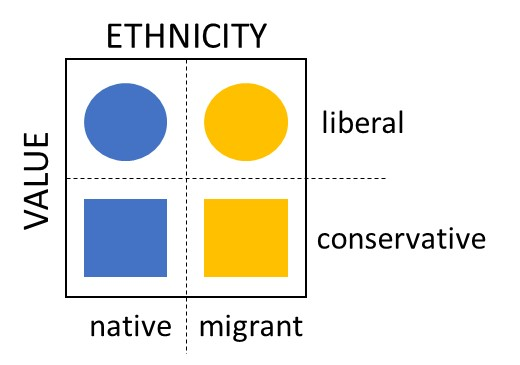
\includegraphics{images/grouptypes.jpg}
    \caption{Agents group-type}
    \label{fig:grp}
\end{figure}

Agents' decision to relocate is modeled as a binary discrete choice random utility model. At each time step, each agent computes the utility of their current cell and an alternative empty one and selects the best one. The utility of each cell depends on the value and ethnic composition of their Moore neighborhood, i.e. the set of their 8 surrounding cells. A cell with not any agent in their Moore neighborhood is set with utility equal to 0, meaning each agent wants to relocate close to at least one similar agent. For each agent, the utility of each cell $i$ is computed as an additive random utility model:

\begin{equation}\label{eq:utot}
U_{i} = \beta_{e}U^{e}_{i} + \beta_{v}U^{v}_{i} +  \epsilon_{i}
\end{equation}

where:\\
$\beta_{e}$: determinism for ethnic preference\\
$E_{i}$: ethnic utility, computed as the proportion of agents of the same ethnicity in the neighborhood of cell $i$, with $U^{e}_{i}=[0,1]$ \\
$\beta_{v}$: determinism for value preference \\
$V_{i}$: value utility, computed as the proportion of agents of the same value orientation in the neighborhood of cell $i$, with $U^{v}_{i}=[0,1]$ \\
$\epsilon_{i}$: random term for selection of cell $i$\newline


The first two terms of the equation represent the systemic utility for cell $i$, while the random term $\epsilon_{i}$ represents any aspect that could influence the relocation choice independent of systemic utility. The higher the parameters of determinism $\beta_{e}$ or $\beta_{v}$, the more likely the selection between the current and the alternative option is based on which one has higher ethnic or value utility. The lower the two parameters, the more likely the selection between the two options is random. The random term is unknown and assumed to follow a type I extreme value distribution, e.g. Gumbel distribution. $\beta_{e}$ and $\beta_{v}$ are numerical parameters we manipulate in our model, imposing a dominant $\beta$ preference and a secondary $\beta$ preference, which depends on the value-orientation of agents. For liberal agents, value $\beta_{v}$ is the dominant preference over ethnic homophily, while for conservative agents ethnic $\beta_{e}$ is the dominant preference over value homophily. The dominant preference for each group-type is a tunable parameter in our model. Secondary preference is a product of dominant preference $\beta_{dom}$ and a weight $w_{sec}$ given to the secondary preference:

\begin{equation}\label{sec}
    \beta_{sec} = \beta_{dom} * w
\end{equation}

Weight $w_{sec}$ ranges from 0 to 1 in step of 0.1, which means that the secondary preference ranges from 0 ($w_{sec} = 0$) to be at most equal to the dominant preference ($w_{sec} = 1$), but never more than the dominant preference.\newline

We implement the inclusion of the random term and the probabilistic decision of agents to relocate from their current cell $cr$ to the alternative cell $al$ with an adapted version of the softmax function\footnote{The softmax function models the probability to select the alternative option $al$ over current option $cr$ is $P_{al} = \frac{\exp(U_{al})}{\exp(U_{al}) +  \exp(U_{cr})}$. The formulation we adopt is a simplified and more computationally efficient version, computed by dividing the numerator and denominator by the numerator, see \citep[p.39]{train2009discrete} for details}. 

\begin{equation} \label{eq:pal}
    P{al} = \frac{1}{ 1 + \exp((\beta_{e}U^{e}_{cr} + \beta_{v}U^{v}_{cr}) - (\beta_{e}U^{e}_{al} + \beta_{v}U^{v}_{al}))}
\end{equation}\newline

As outcomes of our simulations, we report the average exposure index as a measure of segregation and the average density of the neighborhoods agents form.
The exposure index for each agent is the percentage of other similar agents either for ethnic membership or value-orientation in their Moore neighborhood. A condition of segregation occurs when the percentage of similar agents in the neighborhood is higher than that expected if the population were randomly even distributed in the neighborhoods. For an agent $j$, ethnic exposure $E_{j}$ and value exposure $V_{j}$ in our model:

\begin{equation} \label{eq:exposure}
E_{j} = \frac{x^{e}_{j}}{X_{j}}  \quad\text{;}\quad 
V_{j} = \frac{x^{v}_{j}}{X_{j}}
\end{equation}
where:\\
$x^{e}_{j}$: other agents in Moore neighborhood with same ethnicity of agent $j$\\
$x^{v}_{j}$: other agents in Moore neighborhood with same value-orientation of agent $j$\\
$X_{j}$: total other agents in Moore neighborhood\newline

The index is computed for agents with at least one other agent in their neighborhood.\newline
Density of the neighborhood of agent $j$ is the amount of full cells, each occupied by one agent, in their 8 cells Moore neighborhood:

\begin{equation}\label{density}
D_{j} = \frac{X_{j}}{8}
\end{equation}
where:\\
$X_{j}$: total other agents in Moore neighborhood\newline

\hypertarget{Analytical Strategy and Results}{%
\section{Analytical Strategy and Results}\label{results}}


\subsection{Baseline condition: effects of dominant preferences}

In this first section, we are interested in the effect of dominant and secondary preferences of liberal and conservative agents. To this aim, we explore equal sizes conditions where each group-type represents the $25\%$ of the population, so that emerging outcomes can be due only to preferences manipulated. Fig. \ref{fig:landscape} maps an overview of experiments in this section to the space model. For this and the next section, we repeated simulations for 20 runs and collected emerged results at time-step 1000, which was enough to reach stable equilibria. As for parameters of determinism $\beta$, we included levels between 0 to 20 as highest level of determinism\footnote{$\beta$ parameter in random utility models has range $(-\infty,\infty)$. With the need to set a limit to the parameter, we select 20 as enough to observe stable outcomes. We explored higher levels when verifying the model, and not differences were detected. Similarly for the 1000 time-step selection, longer time did not produce differences.}. Results here reported are the average of conditions results.

\begin{figure}
    \centering
    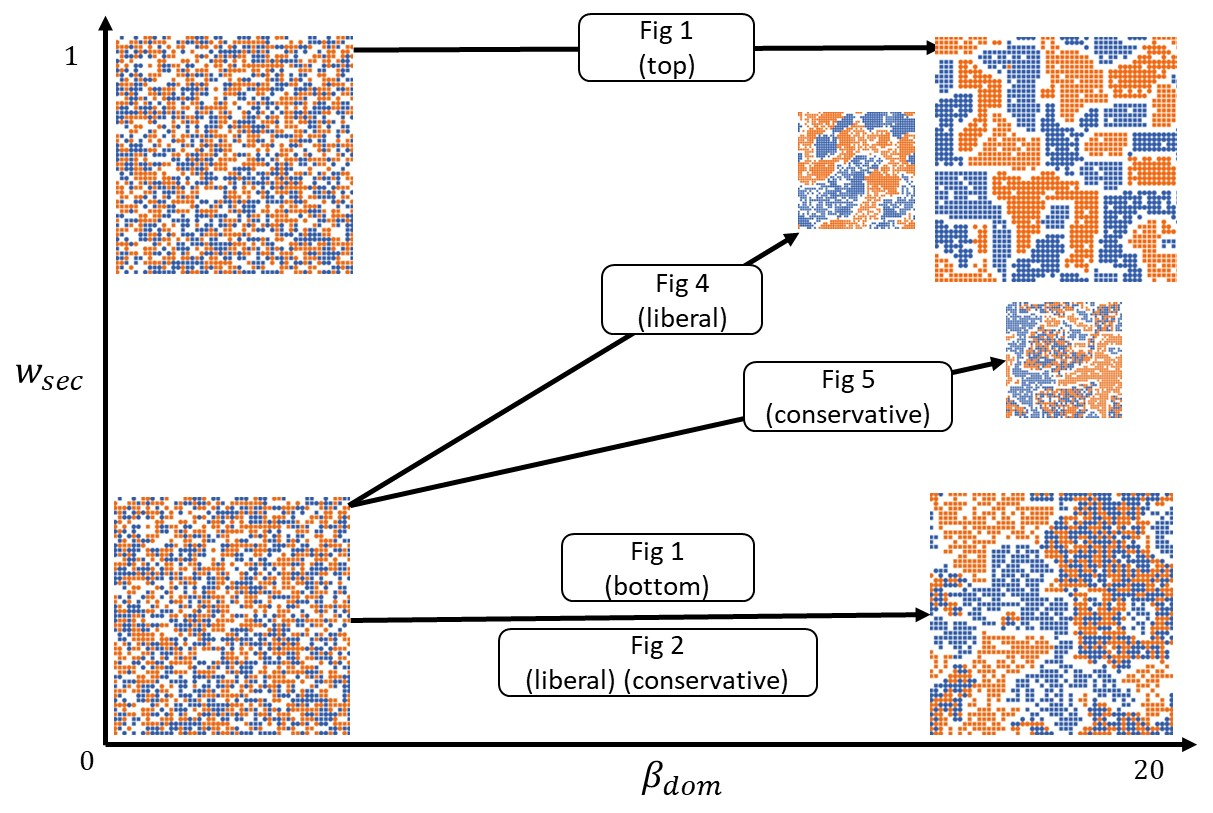
\includegraphics[width = \textwidth]{images/landscape.jpg}
    \caption{Baseline conditions space model and figures overview}
    \label{fig:landscape}
\end{figure}

In Fig.\ref{fig:bsl} we compare the two extreme conditions where agents subscribe to both dominant and secondary preference (top figure, $w_{sec} = 1$) or only to their dominant preference (bottom figure, $w_{sec} = 0$, to explore where stable patterns of double value and ethnic segregation emerge and how scenarios would differ if agents only subscribe to their main preference. The top figure of Fig.\ref{fig:bsl} shows that double segregation would increase linearly until $\beta \approx 5$, while density of neighborhood remains on its baseline. When agents only hold to their dominant preference, segregation and density equilibria are reached at higher levels of determinism $\beta$, while the most interesting outcome is the different outcome of liberals and conservatives. Liberals become segregated by value similarity as their value preference increases, as expected, while they do not differ from the initial random spatial distribution for ethnic exposure. Therefore, they cluster in neighborhoods homogeneous for the secondary dimension of value-orientation, but ethnically mixed between the two groups. On the contrary, conservative agents end up in neighborhoods both ethnically and value segregated, which is incoherent with their preference, because they should segregate only for the ethnic membership according to their  dominant preference. Furthermore, while the density of liberal agents increases as their preferences increase, the density of conservatives decreases compared to the baseline in the top figure.

\begin{figure}[H]
    \centering
    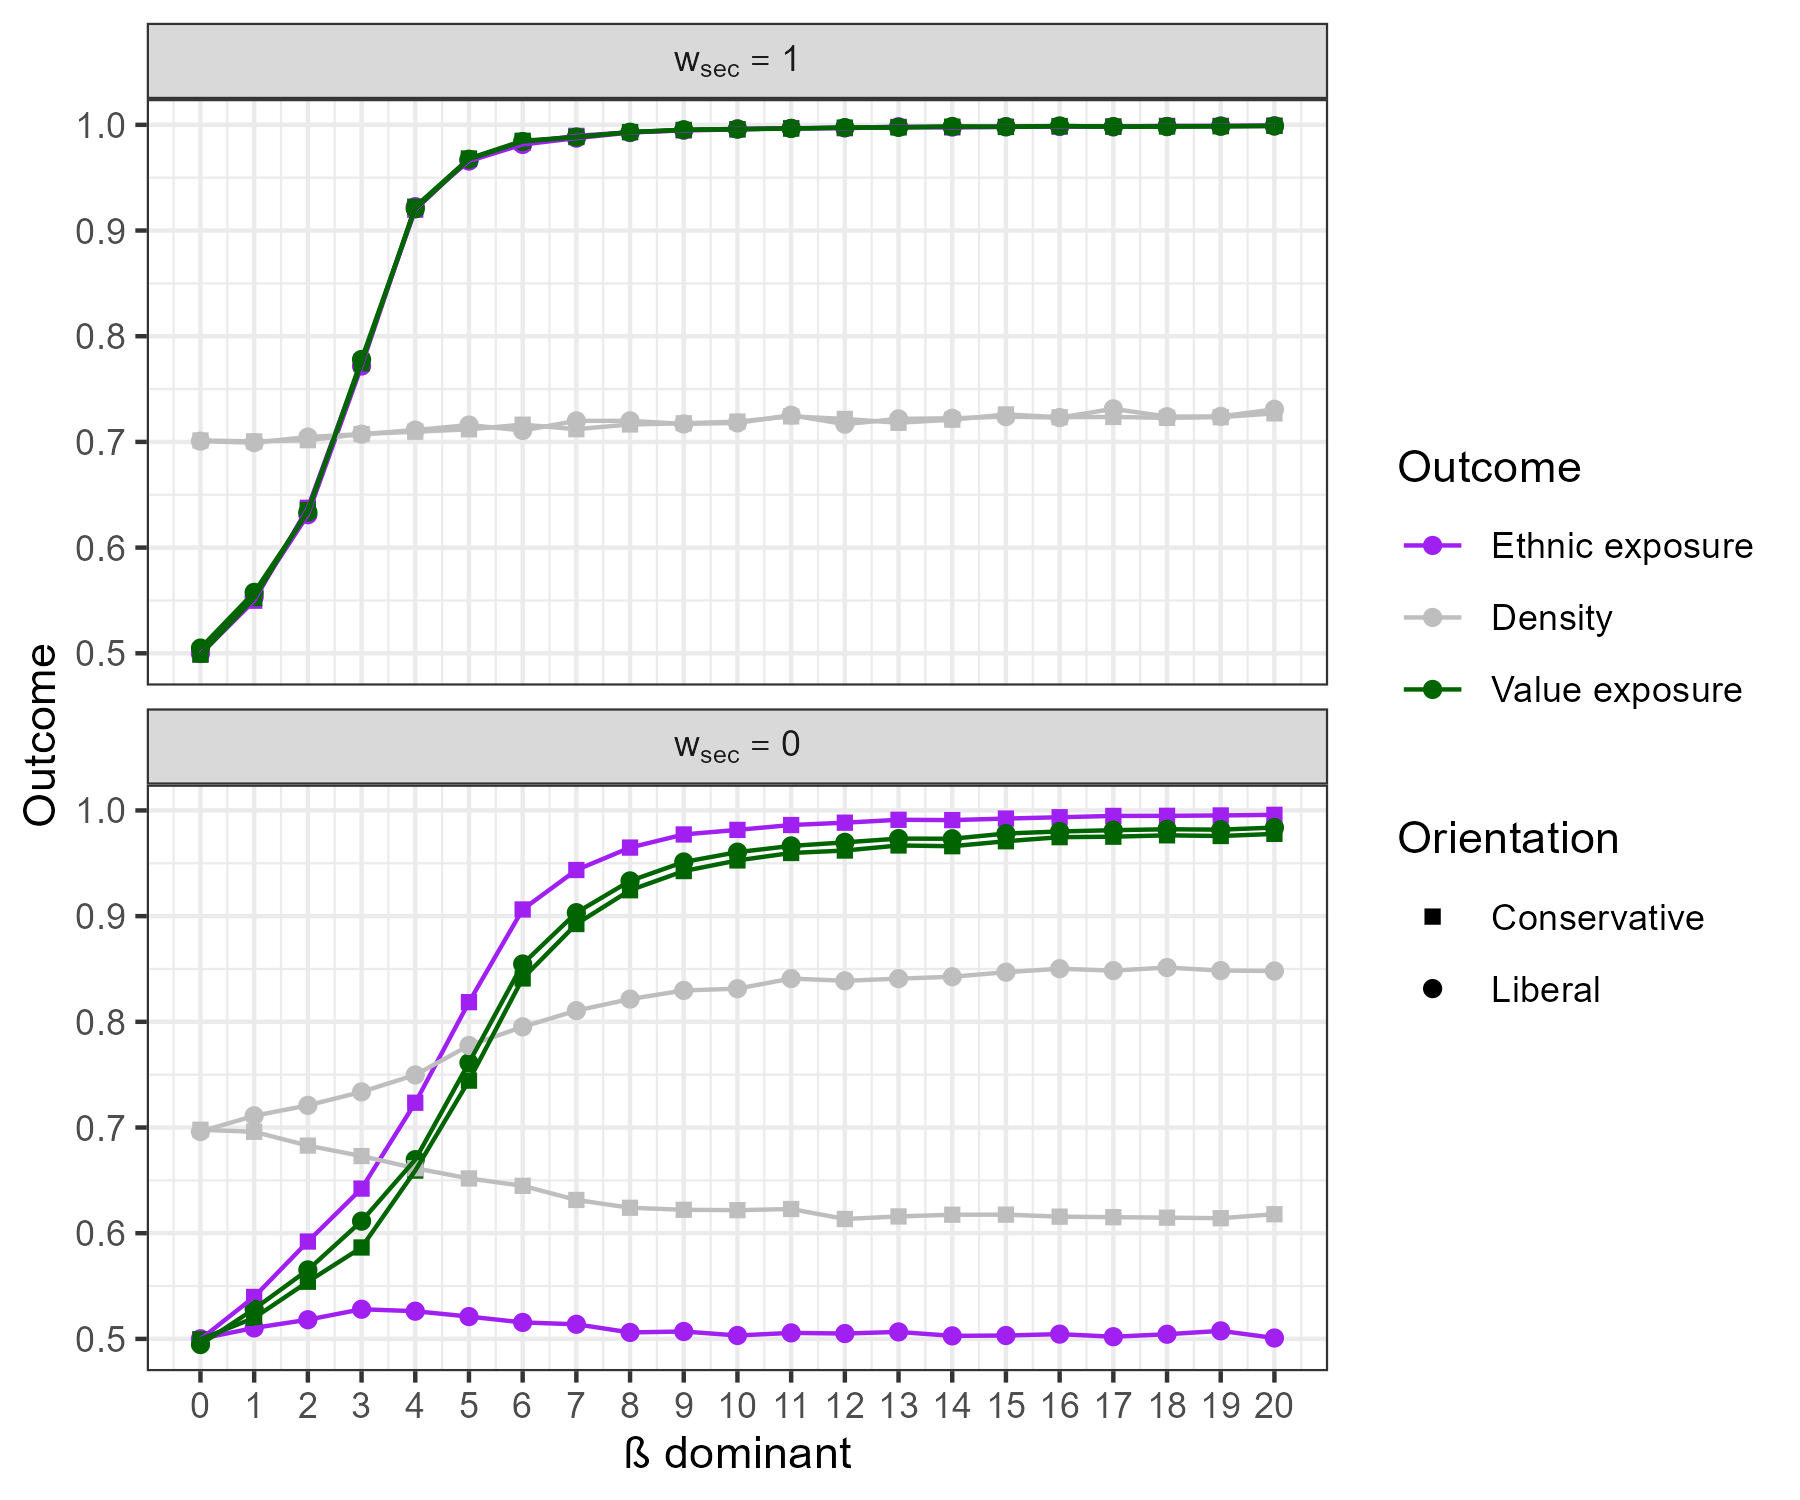
\includegraphics{images/baseline.jpg}
    \caption{baseline}
    \label{fig:bsl}
\end{figure}

 Since agents hold the same degree of determinism in these conditions, it is difficult to disentangle if the different outcomes of liberals and conservatives, in particular the unexpected value segregation of conservatives, are an effect of the own group or the other group, or an interaction of both. Fig.\ref{fig:totsens} clarifies this aspect, by comparing the effect of value preference of liberals over the effect of ethnic preference of conservatives (top figure), and vice versa the effect of ethnic preference of conservatives over the effect of value preference of liberals (bottom figure). The effect of the other group is tested by comparing the same cases under the condition of random relocations of the other group ($\beta = 0$) or high determinism ($\beta = 20$). The comparison shows how value preferences of liberals have an effect on the behavior of conservatives. In particular, when liberals relocate randomly ($\beta$ value liberal = 0), value segregation of conservatives do not occurs: a small increase for extreme determinism occurs because of the clustering of conservative co-ethnics as the only agents driven by deterministic choice. When liberals increase their value preference ($\beta$ value liberal = 20), conservatives fully value segregate for all levels of their ethnic preference, while they do not hold any value preference. We describe this effect as a \textit{by-product} value segregation of ethnic-oriented conservatives due to the value preference of liberals. Also differences in the density of neighborhoods are evident. Liberals form denser neighborhoods as their value preference increase (bottom figure), reaching almost full density if conservatives randomly relocated, and lower density with $\beta$ ethnic conservative = 20, though still higher than the baseline 0.7. On the contrary, conservatives would not increase their density from the baseline even when liberals randomly relocate, while they show stable lower density when $\beta$ value liberal = 20. We explain how the density of neighborhoods formed under homophily preferences based on ethnicity or value similarity can explain the by-product value segregation of conservatives. Due to the equal size of the four group-type, both ethnic-oriented conservatives and value-oriented liberals can consider as similar the $50\%$ of the population to maximize their utility. However, while liberals can cluster with co-values of both ethnic groups, the same doesn't stand for conservatives. When they relocate close to liberal co-ethnics to maximize ethnic utility, they would be rejected because of different value-orientation, so they could actually cluster only with other conservative co-ethnics, i.e. $25\%$ of the population. Liberals instead, form denser neighborhoods since they can cluster with a wider percentage of the population from both of the ethnic groups ($50\%$). Such neighborhoods can only increase value utility and are robust to the relocation of conservatives due to the concentration of liberals of both ethnic groups. The result is the tendency of liberals to form one macro-neighborhood fully value segregated as in the condition of $\beta$ ethnic conservative = 0. The condition $\beta$ value liberal = 0 shows how conservatives would not form denser neighborhoods compared to initial distribution when clustering maximizing ethnic utility. The expansion of value homogeneous neighborhoods of liberals limits the space available for relocation to conservatives, which are forced to cluster with other conservatives co-ethnics to maximize their ethnic preference, so to increase ethnic segregation and value segregation as by-product.\footnote{The decrease in density in both $\beta$ value liberal = 20 and $\beta$ ethnic conservative = 20 are due to lack of random relocation of the other type of agents compared to the other conditions.}


 
 \hfill \newline
 

\begin{figure}[H]
    \centering
    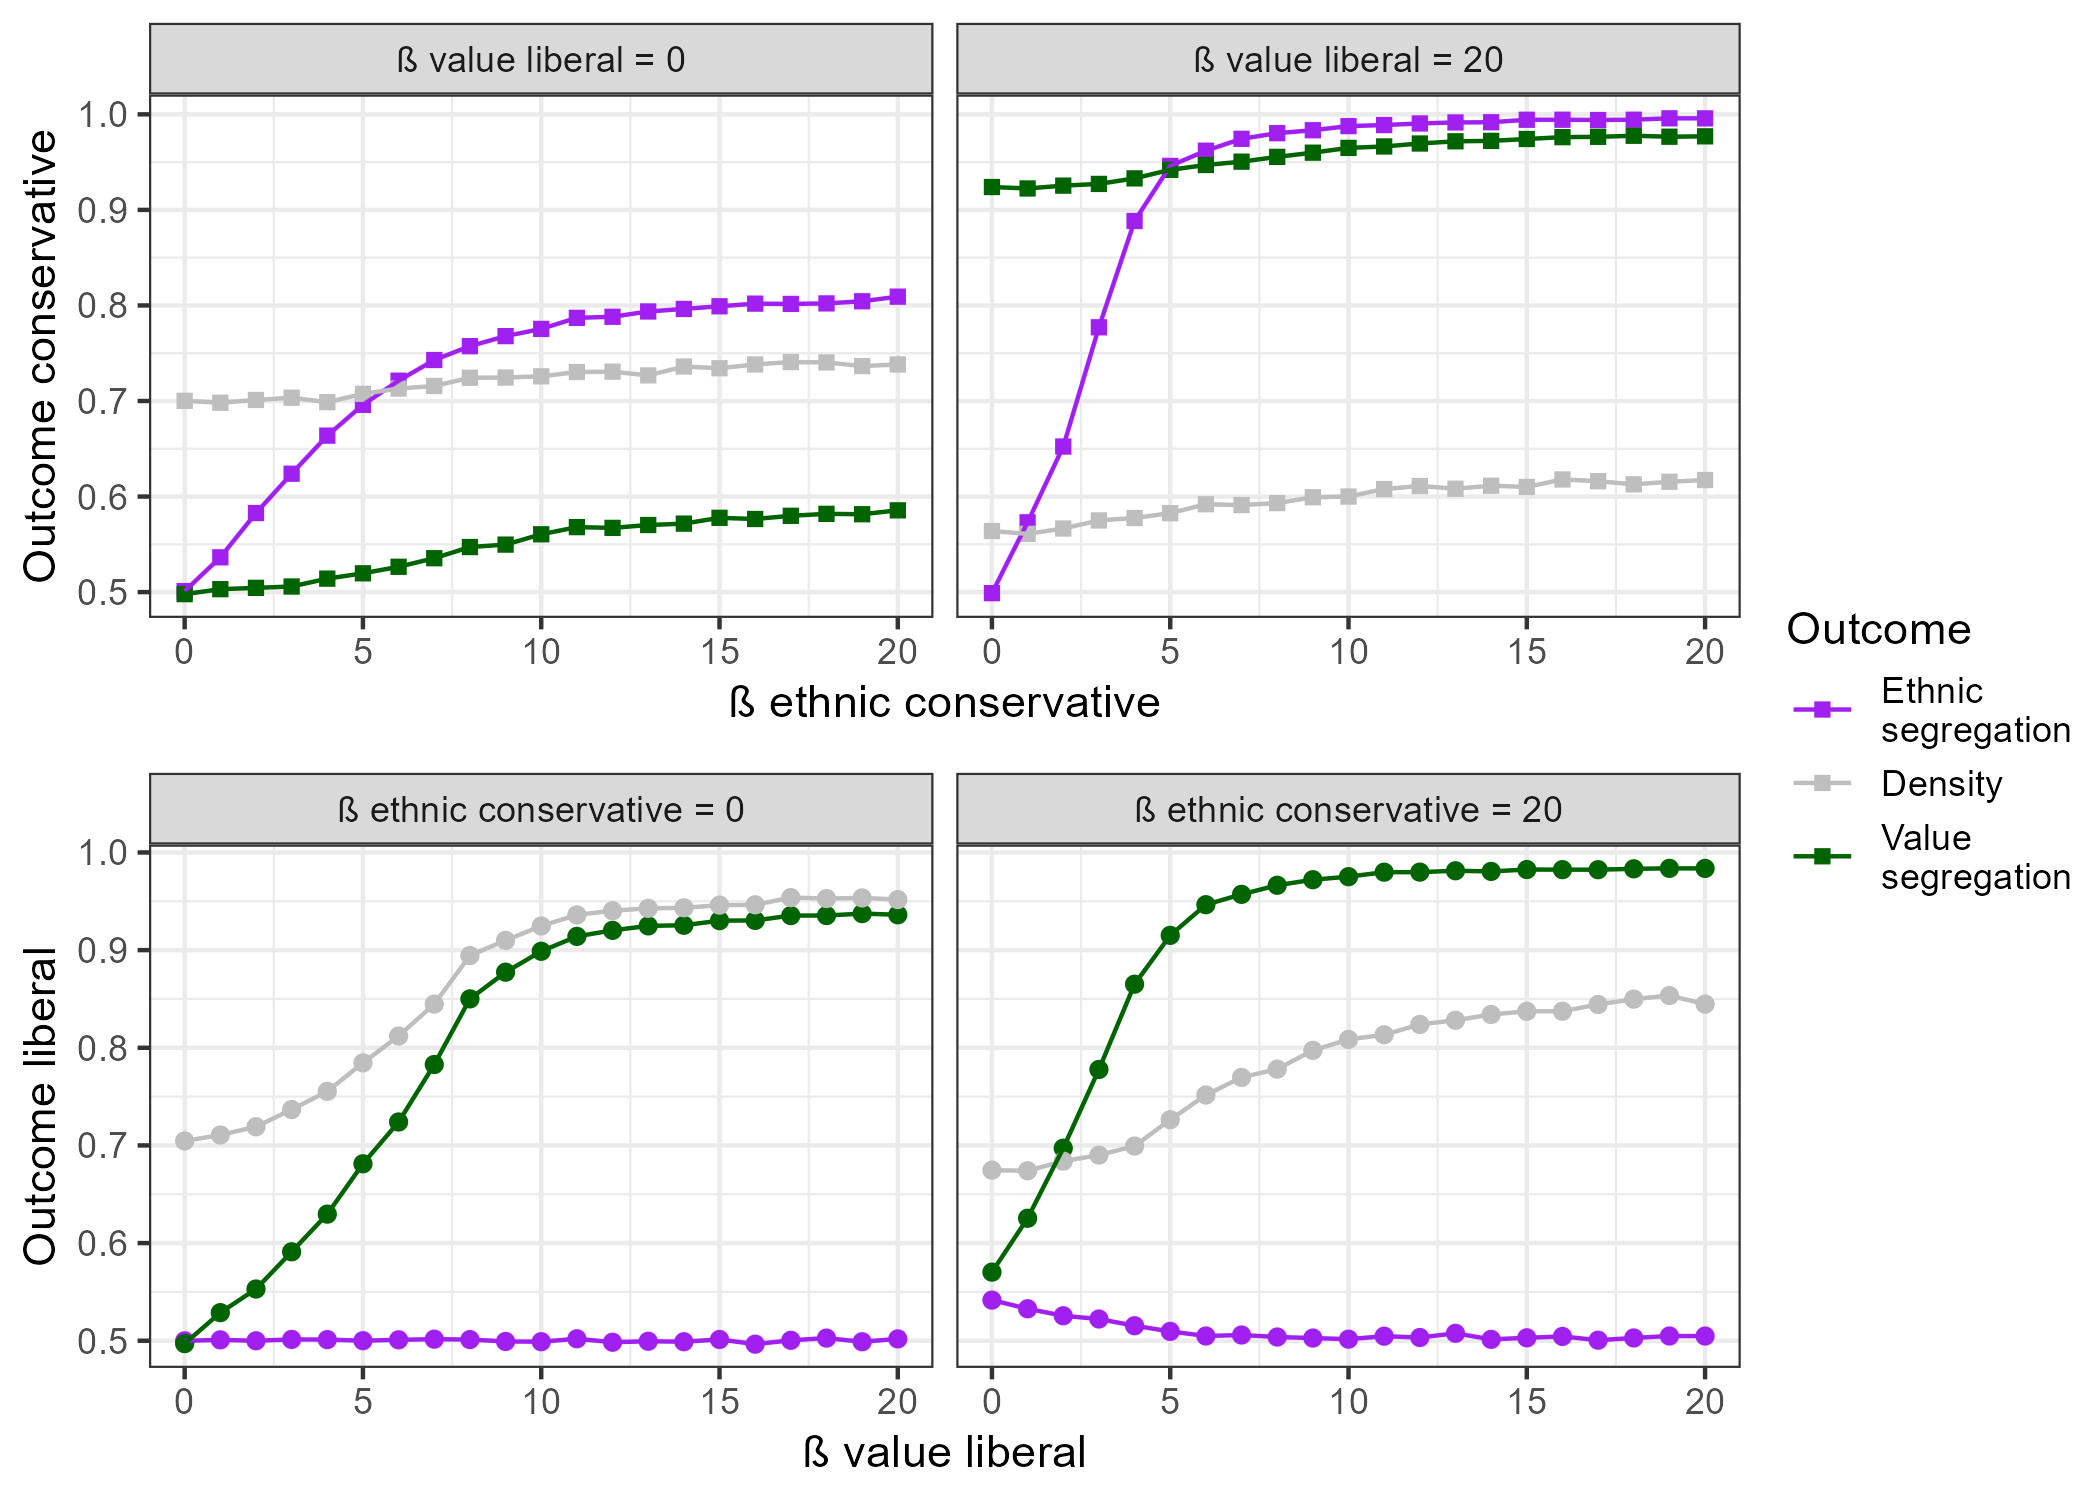
\includegraphics{images/totsens2.jpg}
    \caption{Reciprocal effect of value and ethnic preferences}
    \label{fig:totsens}
\end{figure}


Fig.\ref{fig:libeth} and Fig.\ref{fig:conval} are aimed at investigating how patterns due to different dominant preferences of agents and their interaction showed in the previous figures can change when agents take into consideration also their secondary preferences. We want to test whether an increase in ethnic preferences of liberals can influence the by-product value segregation of conservatives, whether an increase in value preferences of conservatives has an effect, or what other scenarios of hybrid segregation are possible due to the interaction of dominant and secondary preferences for different levels of preference strength. In each figure, dominant preference for both liberal and conservative agents increases up to $\beta = 20$ as in Fig.\ref{fig:bsl}, but we manipulate the parameter $w_{sec}$ for either liberals or conservatives, and report the results for both liberals and conservatives in each scenario. In Fig.\ref{fig:libeth} liberals shift from not holding ethnic preference ($w_{sec} = 0$) to gradually hold same degree of ethnic and value preference ($w_{sec} = 1$); for any level of $w_{sec}$, the dominant value preference on the x-axis is the same. Conservatives in Fig.\ref{fig:libeth} hold only to dominant ethnic preference. Fig.\ref{fig:conval} repeats the experimental condition but with conservatives increasing their value preference as $w_{sec}$ and liberals holding only to value preference for each condition. \newline
In Fig.\ref{fig:libeth}, ethnic segregation of liberals increases as $w_{sec}$ and ethnic preferences increase, as expected, though differences are evident for different degree of determinism. With $w_{sec} < 0.5$, ethnic segregation remains low with small differences between levels of $w_{sec}$, while for higher levels of determinism higher ethnic segregation emerges and differences between the same levels of $w_{sec}$ increase. For $w_{sec} < 0.5$, ethnic utility still has a lower weight, so relocations occur more randomly for the ethnic similarity, while value segregation increases due to value preference. Consider that with $w_{sec} = 0.3$ and dominant value $\beta = 5$ would be equal to 1.5, not enough to generate ethnic segregatio, while for dominant value $\beta = 20$, ethnic $\beta = 6$, which showed in Fig.\ref{fig:bsl} to be enough to allow for stable ethnic segregation. For $w_{sec} \geq 0.5$, the opposite trend emerges: similar levels of full ethnic segregation are reached for higher levels of determinism, and differences more evident for lower value preference determinism. With dominant value $\beta = 0.5$ and $w = 0.5$, ethnic preference would be 2.5, still not enough to cause ethnic segregation, while with $w_{sec} = 1$ both ethnic and value preference would have determinism $\beta = 5$, so that double segregation can emerge. The value exposure of liberals decreases while their ethnic preference increases, because they are more willing to accept conservatives co-ethnic in their group so to increase ethnic utility. For the same reason, the by-product value segregation of conservatives decreases since conservatives can cluster with liberal co-ethnics, showing also an increase in ethnic segregation. Density of liberal agents increase as effect of receiving conservative co-ethnics.

\begin{figure}[H]
    \centering
    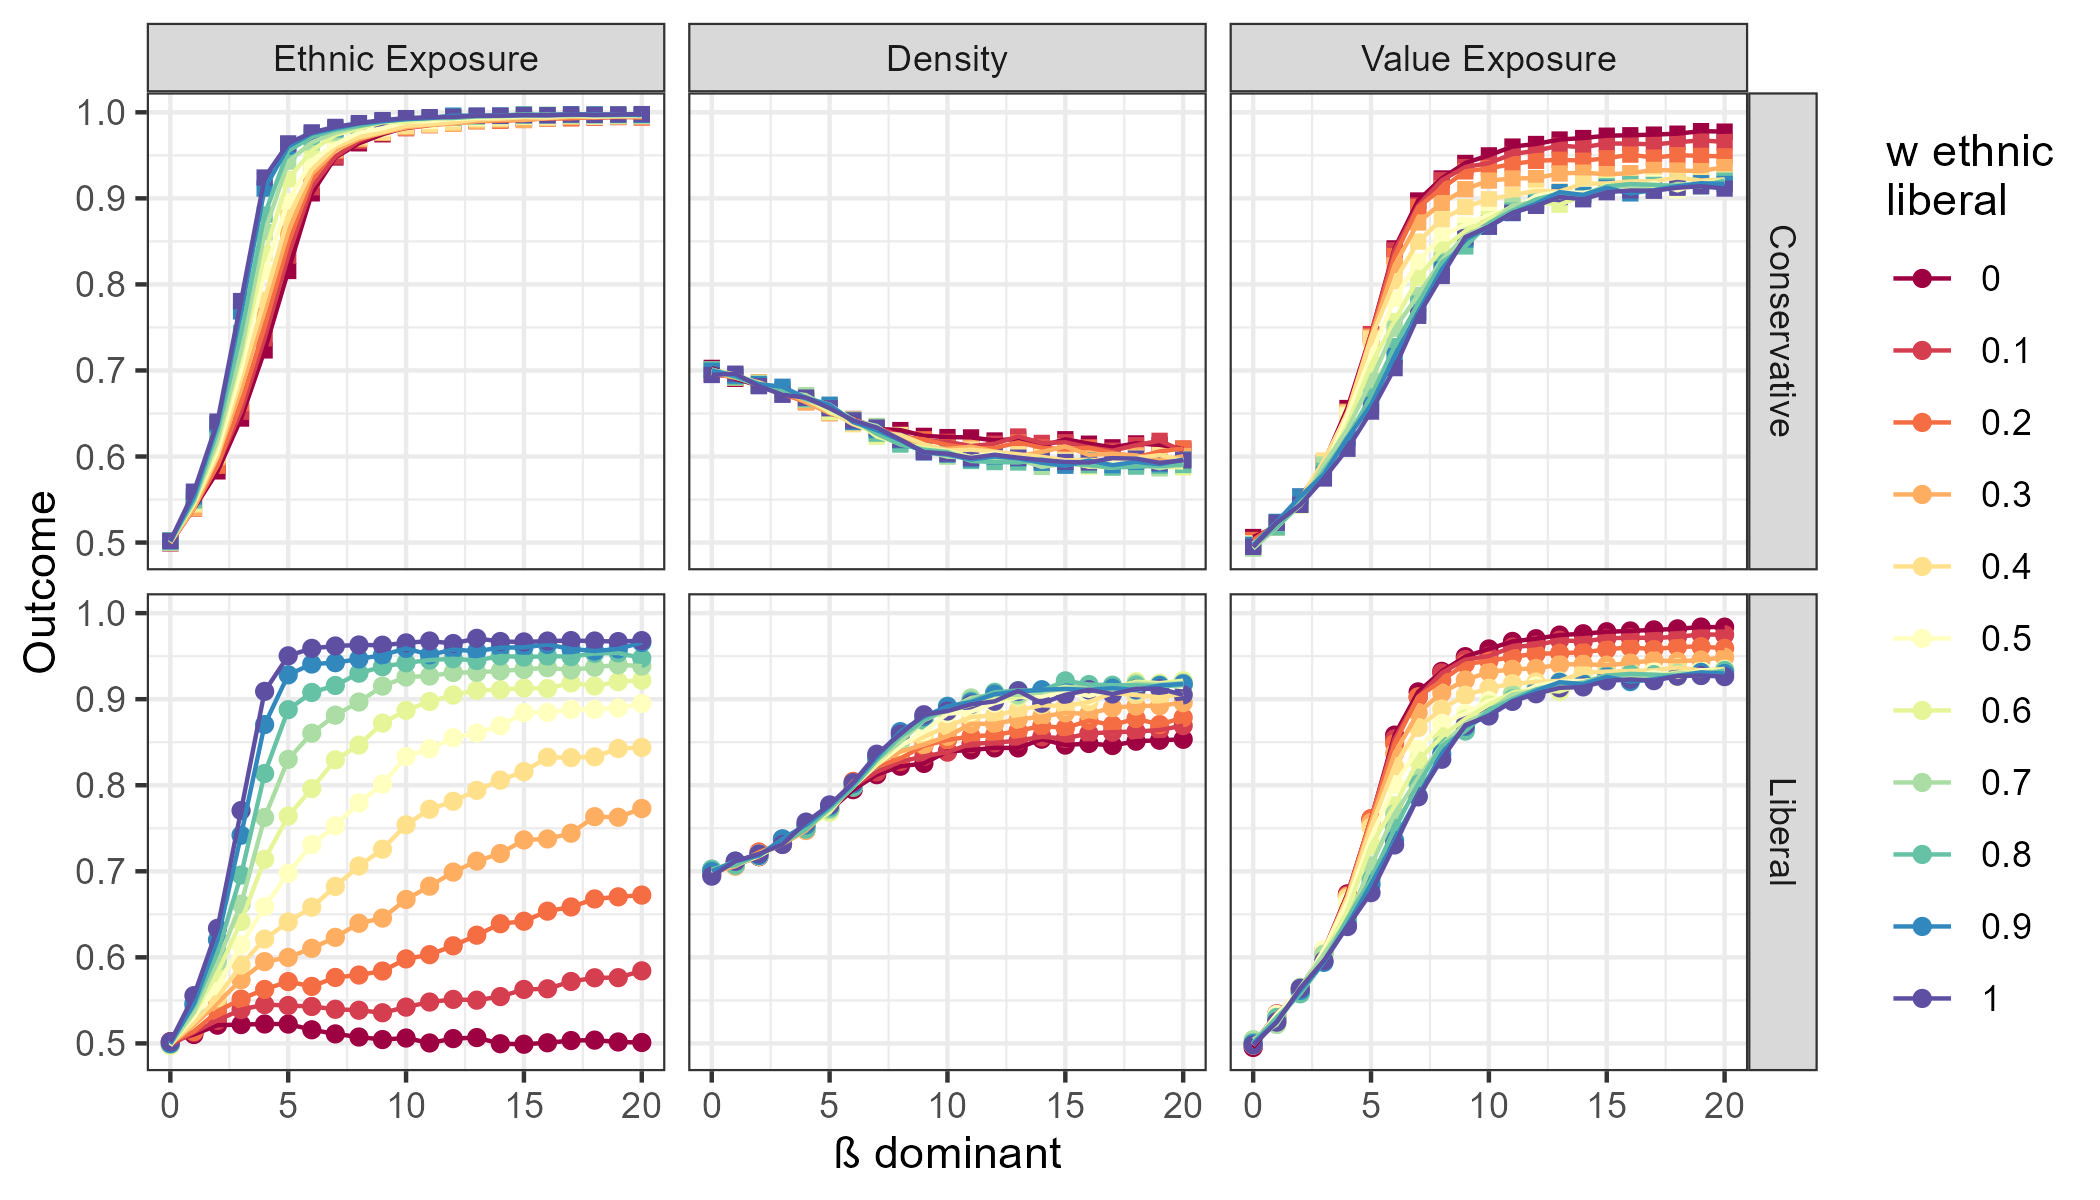
\includegraphics{images/libeth.jpg}
    \caption{Increase in ethnic preferences of liberal agents}
    \label{fig:libeth}
\end{figure}

Fig.\ref{fig:conval} shows how increase in value preferences of conservatives have less effect on the dynamics observed. Conservative increase the density of their neighborhoods that would decrease due to by-product effect of value preferences of liberals, since conservatives would maximize both ethnic and value similarity, so to have less chance to relocate elsewhere. The consequence is a decrease in the density of liberals' neighborhoods, since denser neighborhoods of conservatives would still limit the space to the expansion of liberals' neighborhood. Though, the increase in value preferences of conservatives reinforces the value segregation of liberals, especially in the region of lower determinism, because conservatives will not try to relocate to the edge of liberals' neighborhood to increase their ethnic preferences.

\begin{figure}[H]
    \centering
    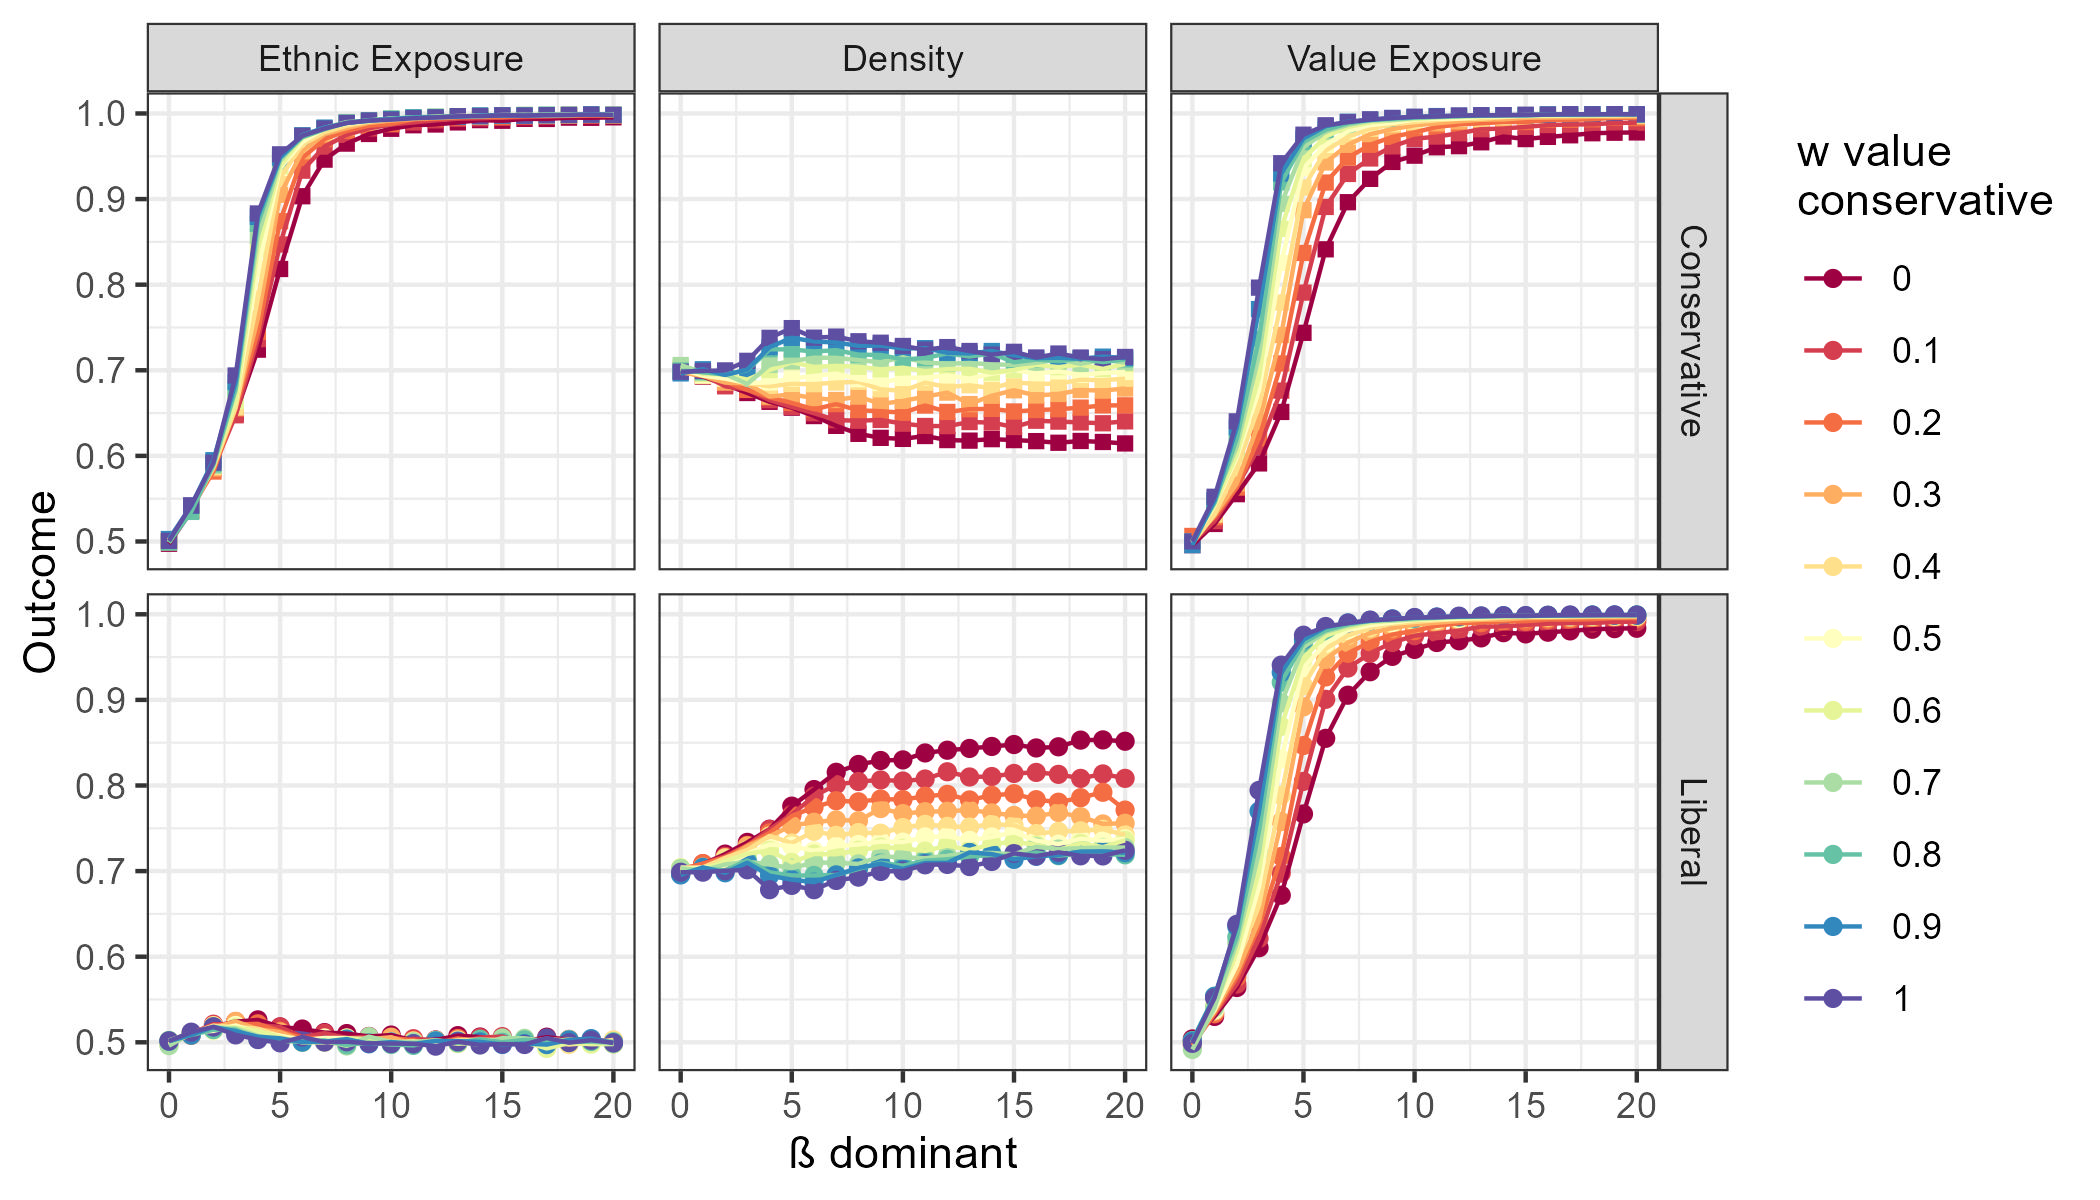
\includegraphics{images/conval.jpg}
    \caption{Increase in value preference of conservative agents}
    \label{fig:conval}
\end{figure}

\subsection{Asymmetric Conditions}

In this section we explore the effect of relative sizes for value distribution. Baseline conditions showed how preferences based on ethnicity and value similarity can influence the reciprocal behavior of conservative and liberal agents, and how increase in secondary preference can modulate the mechanisms observed. We expect the unequal group sizes to show further hybrid scenarios on the continuum between segregation and integration due to the effect on relocations to find similar ones. 

Since major changes in the baseline conditions were caused by the preference of liberal agents, we focus here on the interaction of increasing ethnic preference of liberal agents of both groups, along with the effect of increasing strength of preferences in the condition of asymmetric groups. For sake of simplicity, we present here one condition of asymmetric distribution of liberals within each ethnic group, keeping each ethnic group and each value-orientation equal to $50\%$ of the global population (see left side of Fig.\ref{fig:asymlndscp}):  $40\%$ liberal natives, $10\%$ conservative natives, $10\%$ liberal migrants, $40\%$ conservative migrants. We studied also other conditions of relative sizes we report in the Annex we will refer to.\footnote{In the annex we report 2 conditions: a majority/minority condition and a minority/minority condition. In the majority/minority condition, we manipulate the ethnic ratio (from $50\%$ native and $50\%$ migrant to $80\%$ natives and $20\%$ migrants) keeping $50\%$ of liberals in each ethnic group. In the minority/minority condition, reported in the manuscript, each ethnic group represents the $50\%$ of the population, but we impose a probability for liberals in the native ethnic group ($P^{n}_{l}$), and probability of liberals in the minority ethnic group as complement probability to it ($1 - P^{n}_{l}$).} This condition best fits our interests to identify conditions for hybrid segregation for several reasons. First, this scenario is conceptually closer to the paradigm of super-diversity challenging the assumption of majority/minority ethnic condition in modern societies (ref).\footnote{We explore this scenario in Annex and demonstrate how differences are a linear effect of higher numerosity of majority group} Still, the scenario can reflect the stratification of society where higher socio-economic status or higher education can still be higher in the native population and being in a minority group of migrants' descendants \citep{crul2017upcoming}. Importantly, this condition has implications for the mechanisms we observed in the baseline scenario and that we want to put to the test. As in the baseline scenario, each agent has an equal probability to find a similar one for both ethnicity and value-orientation. However, in the native population liberals are in the majority condition compared to conservative co-ethnics, which might have implications for computed value utility and by-product value segregation of conservatives. Also, conservative natives are the minority of ethnicity-oriented agents. On the other side, liberal migrants represent a minority both in their own ethnic group and compared to liberal natives. Though, liberal migrants could count on $50\%$ of the population if they were to increase ethnic preferences, majority of which conservatives. We expect these conditions to influence the dependencies between emerging outcome of group-types.

We set other conditions as in the figure on the right side of Fig.\ref{fig:asymlndscp}. We increase dominant preferences for both types of agents as in the baseline scenario, but we manipulate independently the weight of secondary ethnic preference for liberal natives ($w^{lm}_{e}$) and liberal migrants ($w^{ln}_{e}$). We select options $w_{sec} = 0$ (liberals only hold to value preferences), $w_{sec} = 1$ (liberals hold to both value and ethnic preferences), and $w_{sec} = 0.5$ has an intermediate condition that is more sensitive to different levels of determinism.




\begin{figure}[H]
    \centering
    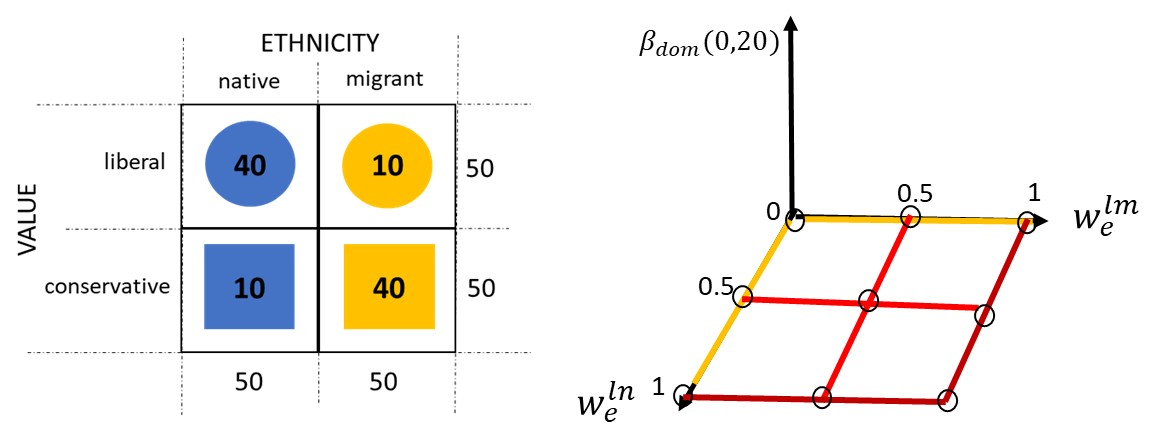
\includegraphics{images/asym_landscape.jpg}
    \caption{On the left the asymmetric conditions explored in this section, on the right, the conditions reported}
    \label{fig:asymlndscp}
\end{figure}

In Fig.\ref{fig:asymnat} we focus on the native population, comparing conservatives (in the minority value condition) and liberals (in the majority value condition). Conservative agents fall into value segregation in the region of lower determinism ($\beta \approx 4$), though they fall again into value segregation as determinism increases, where they become fully ethnic segregated. The reason is that due to their condition of minority, conservative natives need to cluster with liberal co-ethnics to satisfy their ethnic utility. Due to their lower numerosity, liberal natives can tolerate them, in particular in the area of lower determinism, where value preference is still relatively low. A slight reinforce of the ethnic assimilation  occurs when liberal natives also increase their ethnic preferences, so to accept more conservative co-ethnics. When determinism of agents increases, the by-product value segregation of conservatives takes on, though to a lower level compared to baseline conditions due to lower numerosity of conservatives (see annex for a comparison). An interesting outcome is that the by-product value segregation of conservative natives decreases when ethnic preference of liberal migrants increases, and not for the increase in the ethnic preference of liberal natives. When liberal migrants increase their ethnic preferences, they would have equal preference for liberal natives for value utility and conservative migrants for ethnic utility. While both groups would accept liberal migrants, conservative migrants would reject liberal natives because of their ethnicity, while liberal natives would remain close to liberal migrants, who would still prefer other liberal co-ethnics to increase ethnic utility. This creates a cascade of neighborhood formation between groups. Liberal natives form denser neighborhoods both value and ethnic segregated within larger neighborhoods of liberal natives. Value homogeneous neighborhoods of liberal natives become consequently also ethnically segregated. Such neighborhoods attract conservative natives who can increase their ethnic preference relocating close to liberal natives, decreasing value segregation, reinforced when liberal natives also increase their ethnic preference. When liberal migrants hold only to value preferences, value homogeneous neighborhoods of liberals would be ethnically mixed, so that conservative natives can avoid them because of liberal migrants.


\begin{figure}[H]
    \centering
    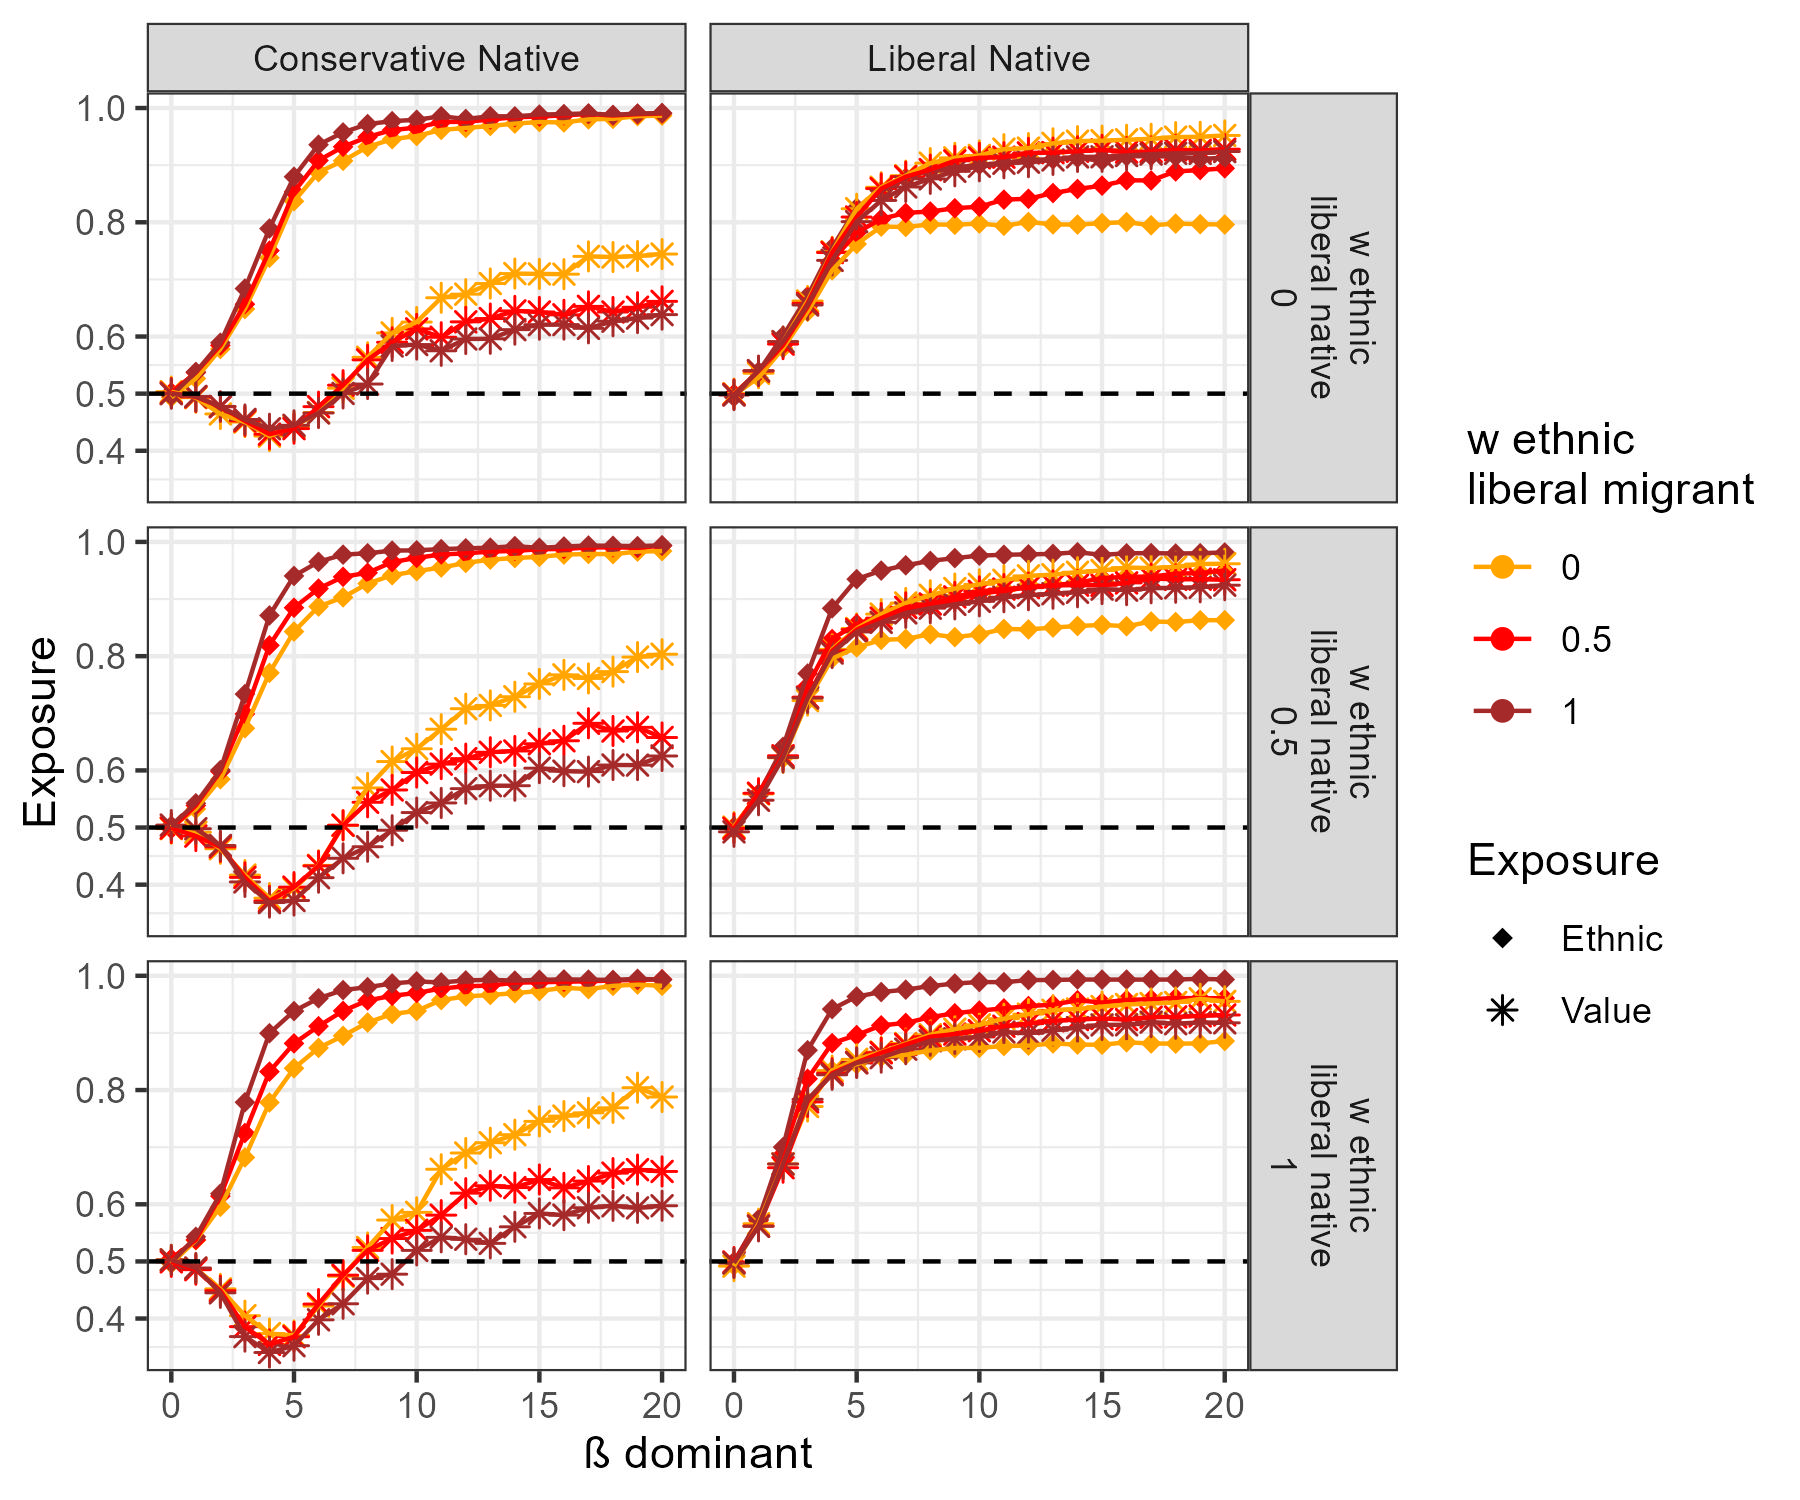
\includegraphics{images/asym_native.jpg}
    \caption{Increase in ethnic preferences of liberals. Native population, comparison of conservative native and liberal native}
    \label{fig:asymnat}
\end{figure}

In Fig.\ref{fig:asymmig}, liberal migrants show more hybrid segregation scenarios compared to conservative natives, in particular with intermediate preferences of $w_{ethnic} = 0.5$. When liberals of both groups only hold to value preferences, ethnic assimilation of liberal migrants occurs, due to being in the minority condition. As the ethnic preference of liberals increases, ethnic exposure increases both for liberal migrants and liberal natives in Fig.\ref{fig:asymnat}. Full ethnic segregation cannot occur because liberal migrants still want to relocate also close to liberal natives. With liberal migrants $w_{ethnic} = 0.5$, the ethnic segregation has a curve shape pattern as determinism increases, below ethic exposure for $\beta \approx 7$ and then above, though remaining close to ethnic integration. For $\beta = 7$, ethnic preference $\beta_{e}$ of liberal migrants is $3.5$, still low but enough to cluster close to more co-ethnics, though preferring more living close to liberals, as high value segregation shows. For $\beta \leq 5$, liberal migrants are both ethnically and value integrated. For high levels of determinism, value segregation is still higher than ethnic segregation, though this increases to 0.7. This is the scenario for decreased by-product value segregation occurs, with value and ethnic segregated neighborhoods of liberal migrants located within larger neighborhoods of liberal natives. When liberal natives increase their ethnic preference, but liberal migrants still hold only to value preference, ethnic segregation of liberal migrants does not occur. In this scenario liberal natives form ethnically and value segregated neighborhoods out of their preferences, though liberal migrants can still be accepted since in a minority condition so to not threat their value utility. When both liberal natives and liberal migrants hold both ethnic and value preferences, value assimilation occurs for liberal migrants for a short window at $\beta \approx 4$ because agents form more mixed neighborhoods due to random relocations, with liberal migrants being in the minority compared to to conservative migrants, and liberal migrants having more likelihood to relocate close to liberal co-ethnic due to higher numerosity. When determinism increases, liberal migrants cluster closer to other liberal co-ethnics.


\begin{figure}[H]
    \centering
    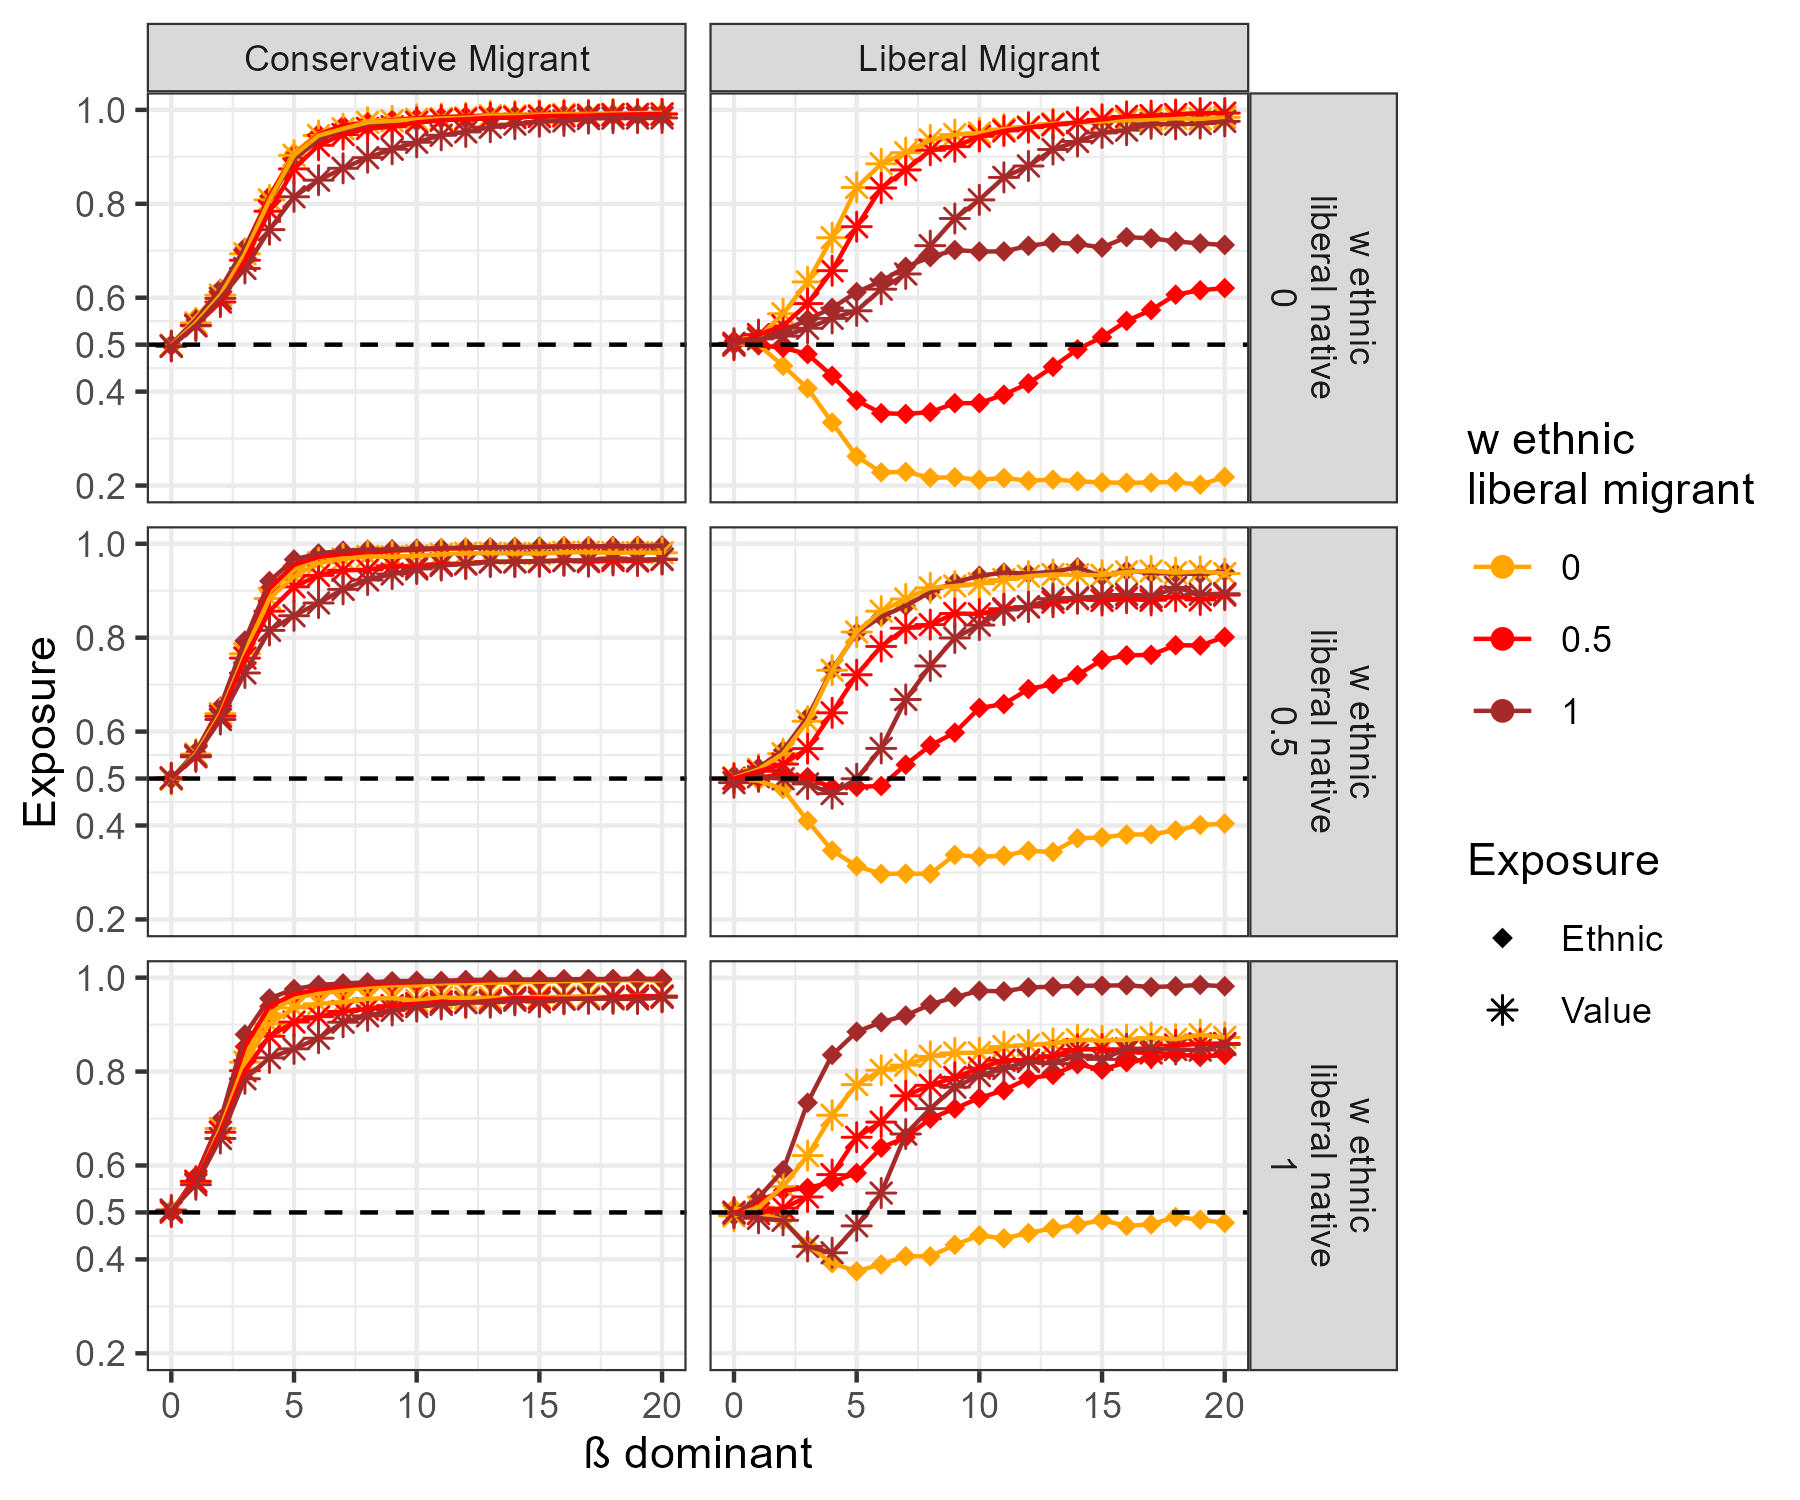
\includegraphics{images/asym_migrant.jpg}
    \caption{Increase in ethnic preferences of liberals. Migrant population, comparison of conservative migrant and liberal migrant}
    \label{fig:asymmig}
\end{figure}

\section{Conclusions and Discussion}

\section{Annex A: Relative group size, minority-minority condition}

\begin{figure}[H]
    \centering
    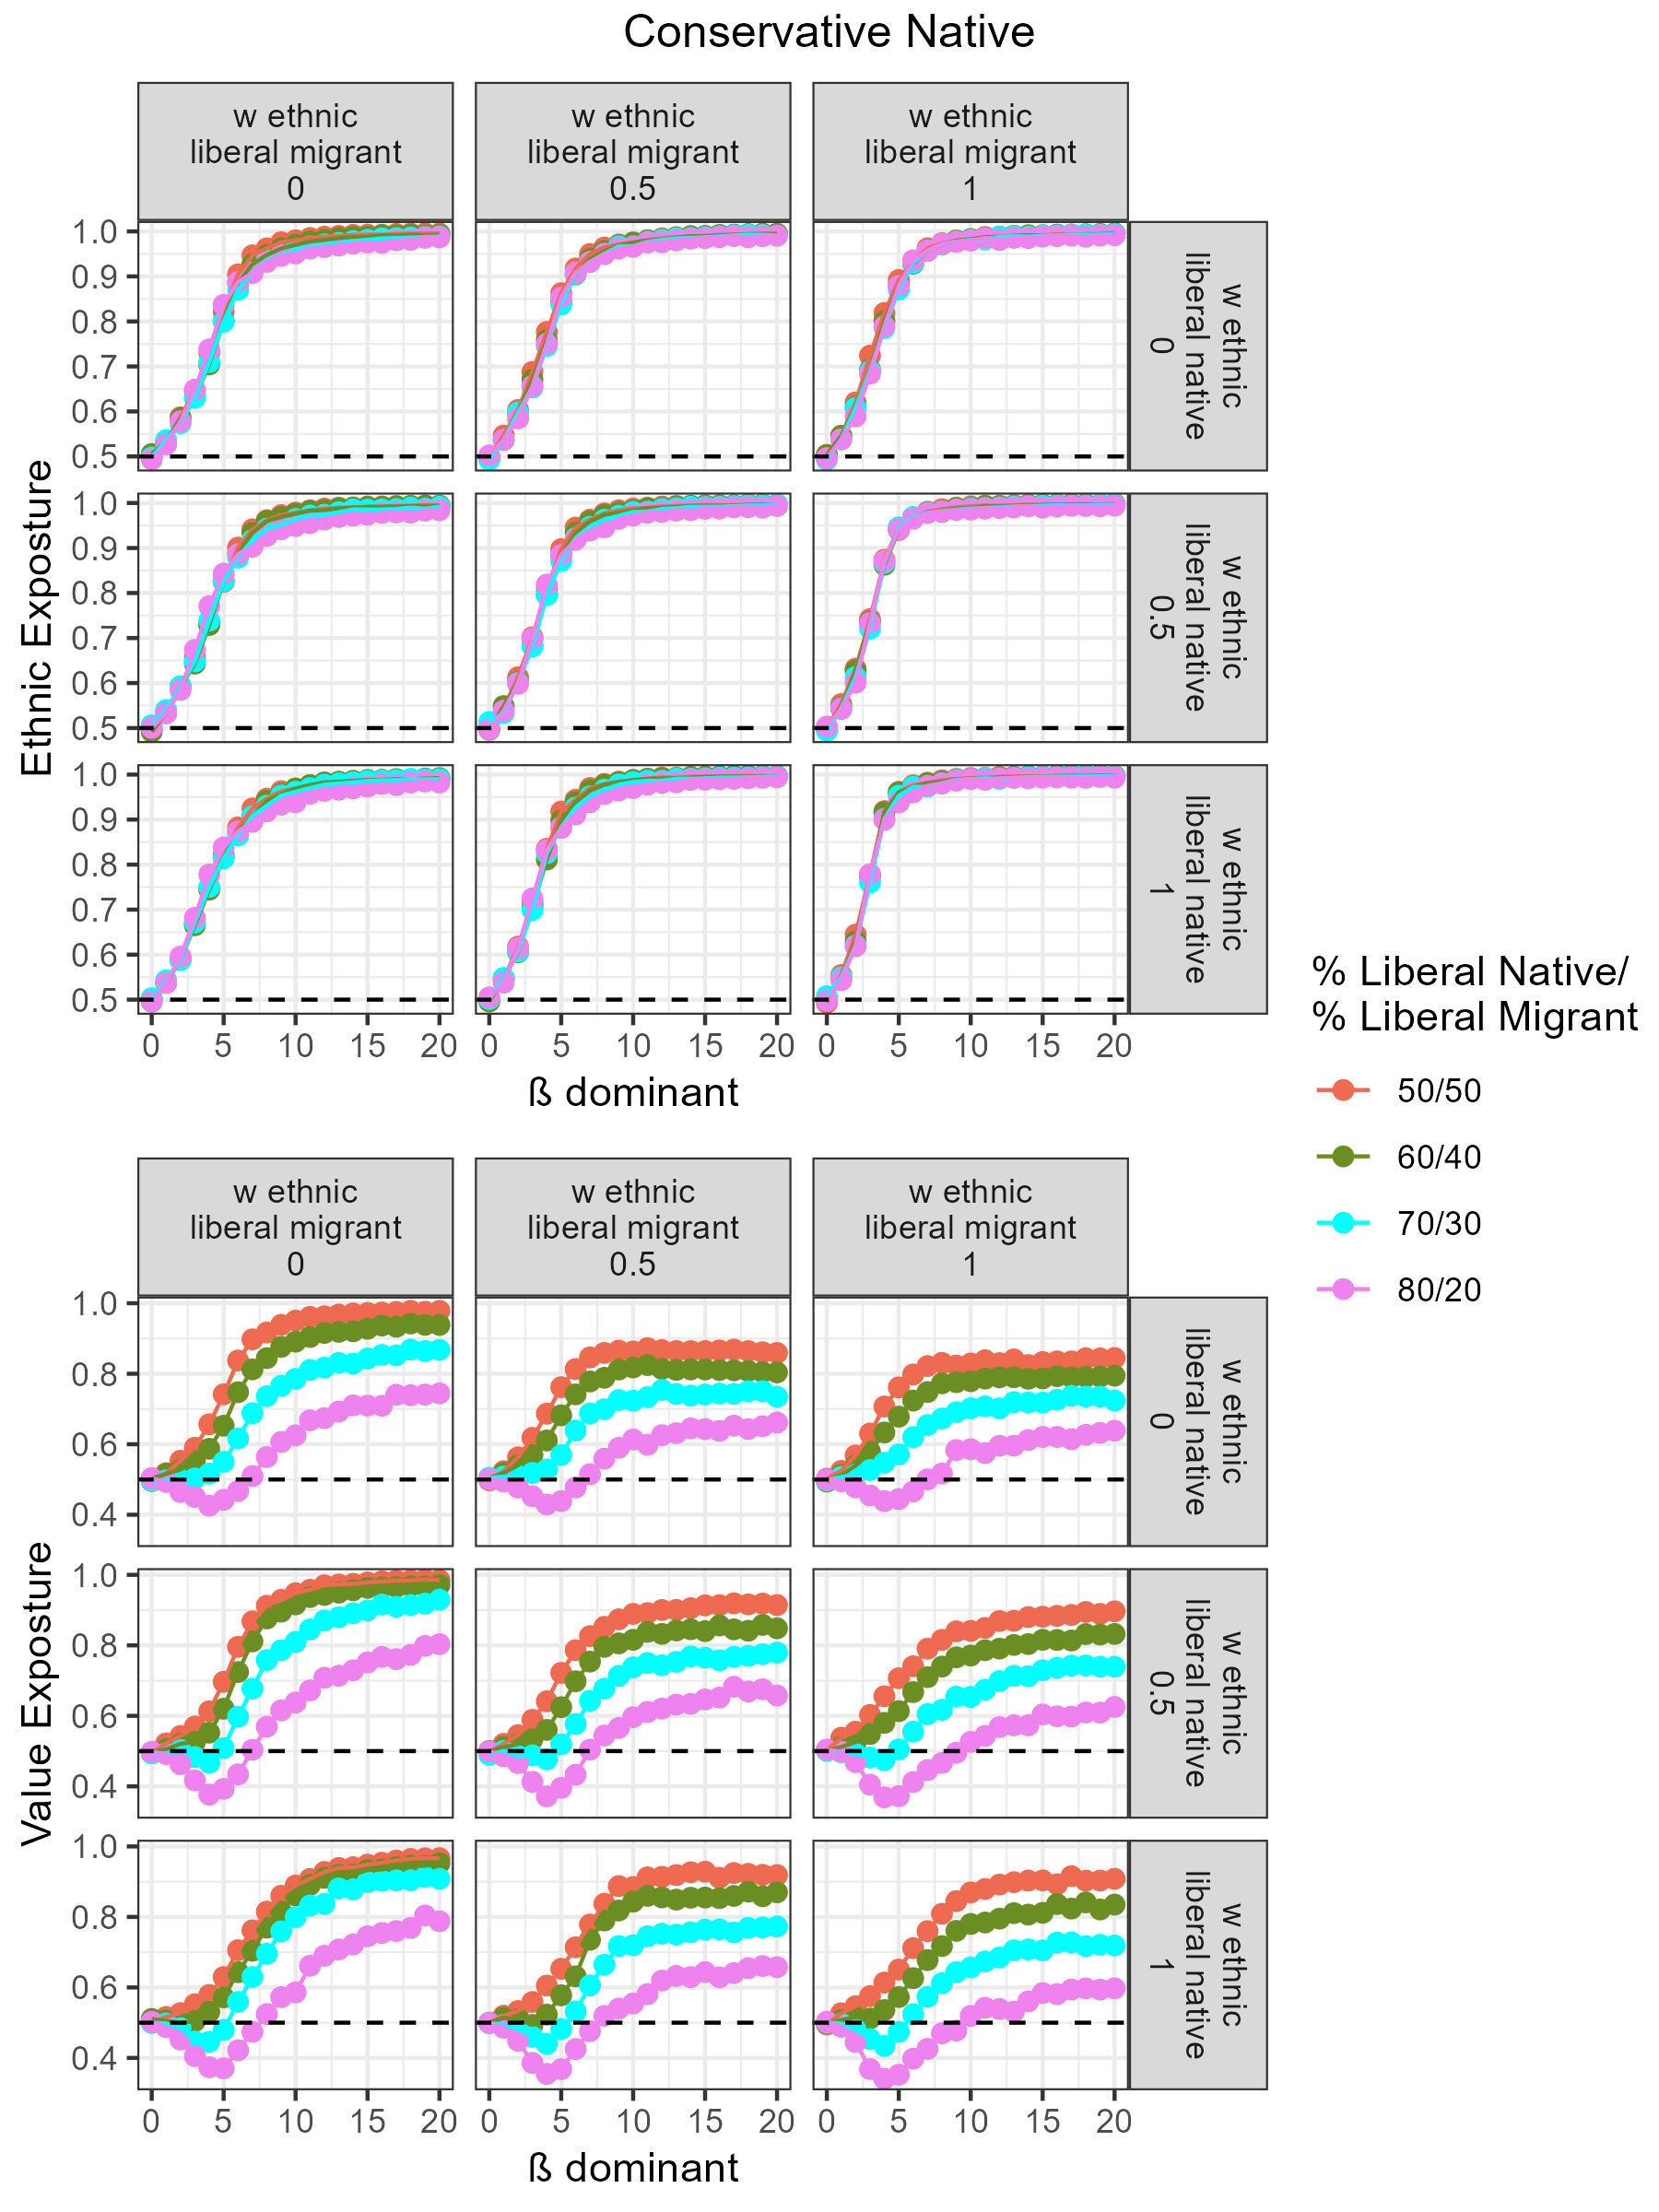
\includegraphics{images/Conservative Native_vlsz.jpg}
    \caption{Conservative native; minority/minority condition}
    \label{fig:consnat}
\end{figure}

\begin{figure}[H]
    \centering
    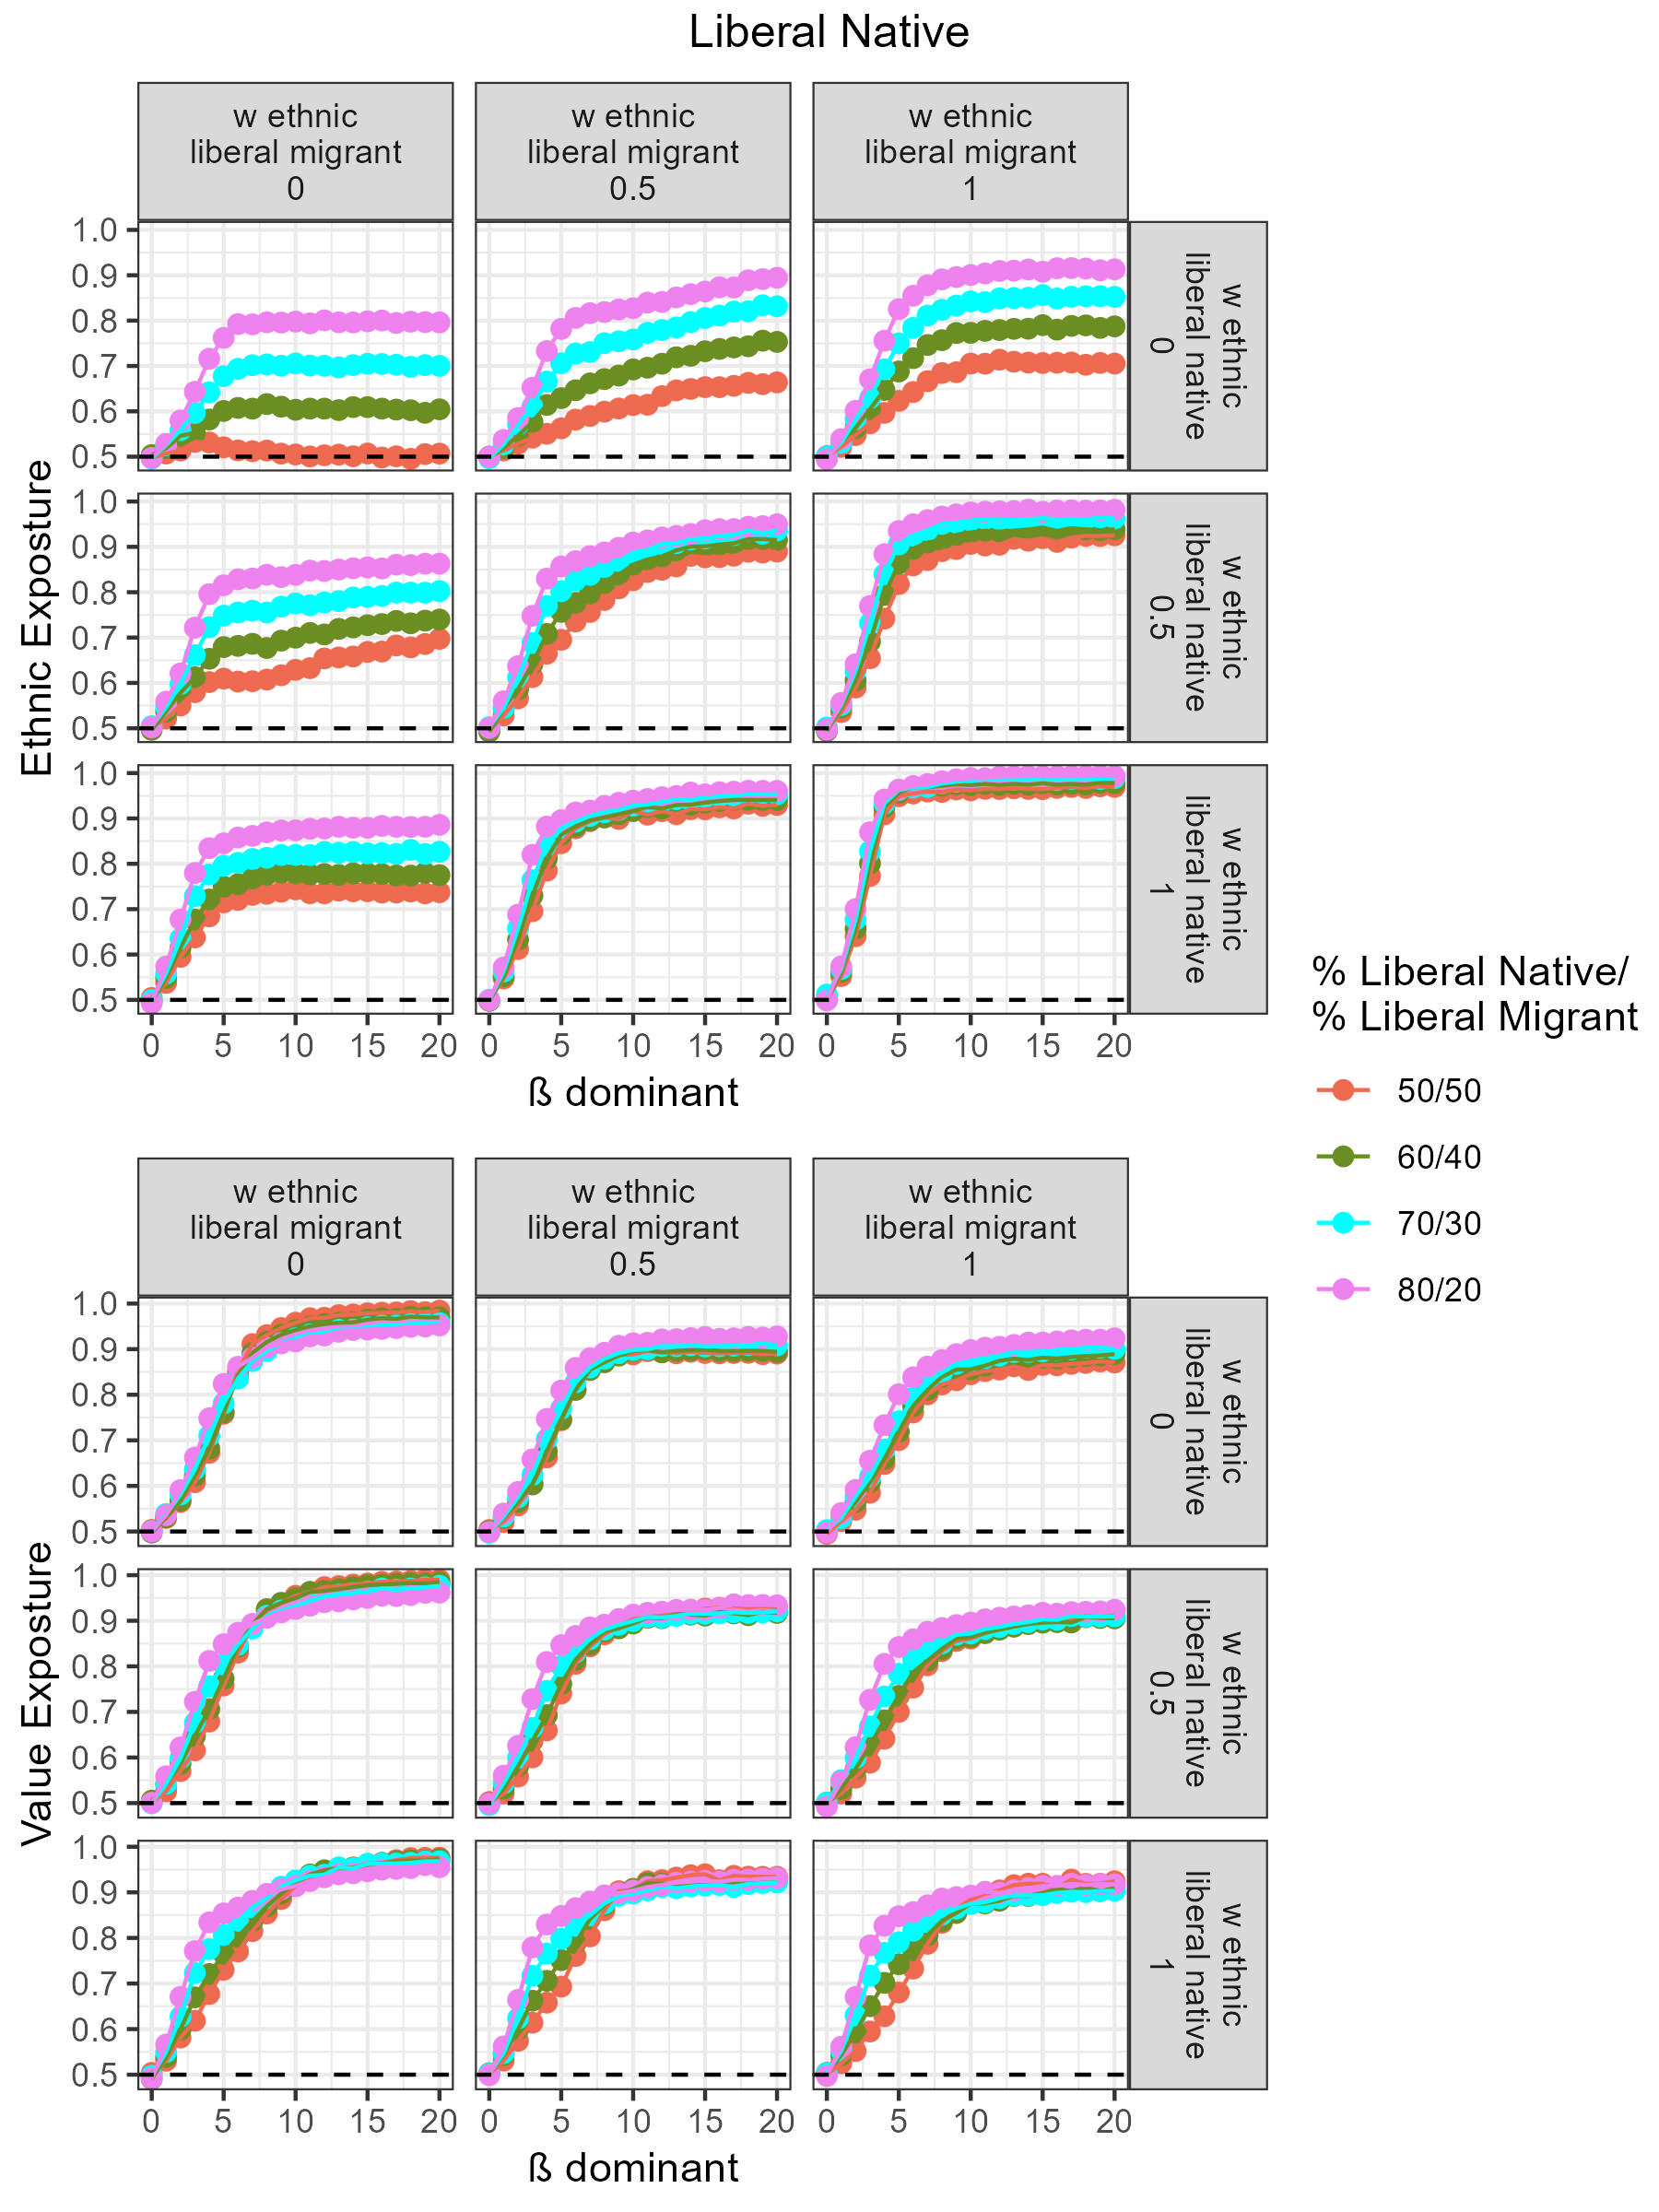
\includegraphics{images/Liberal Native_vlsz.jpg}
    \caption{Liberal native; minority/minority condition}
    \label{fig:libnat}
\end{figure}

\begin{figure}[H]
    \centering
    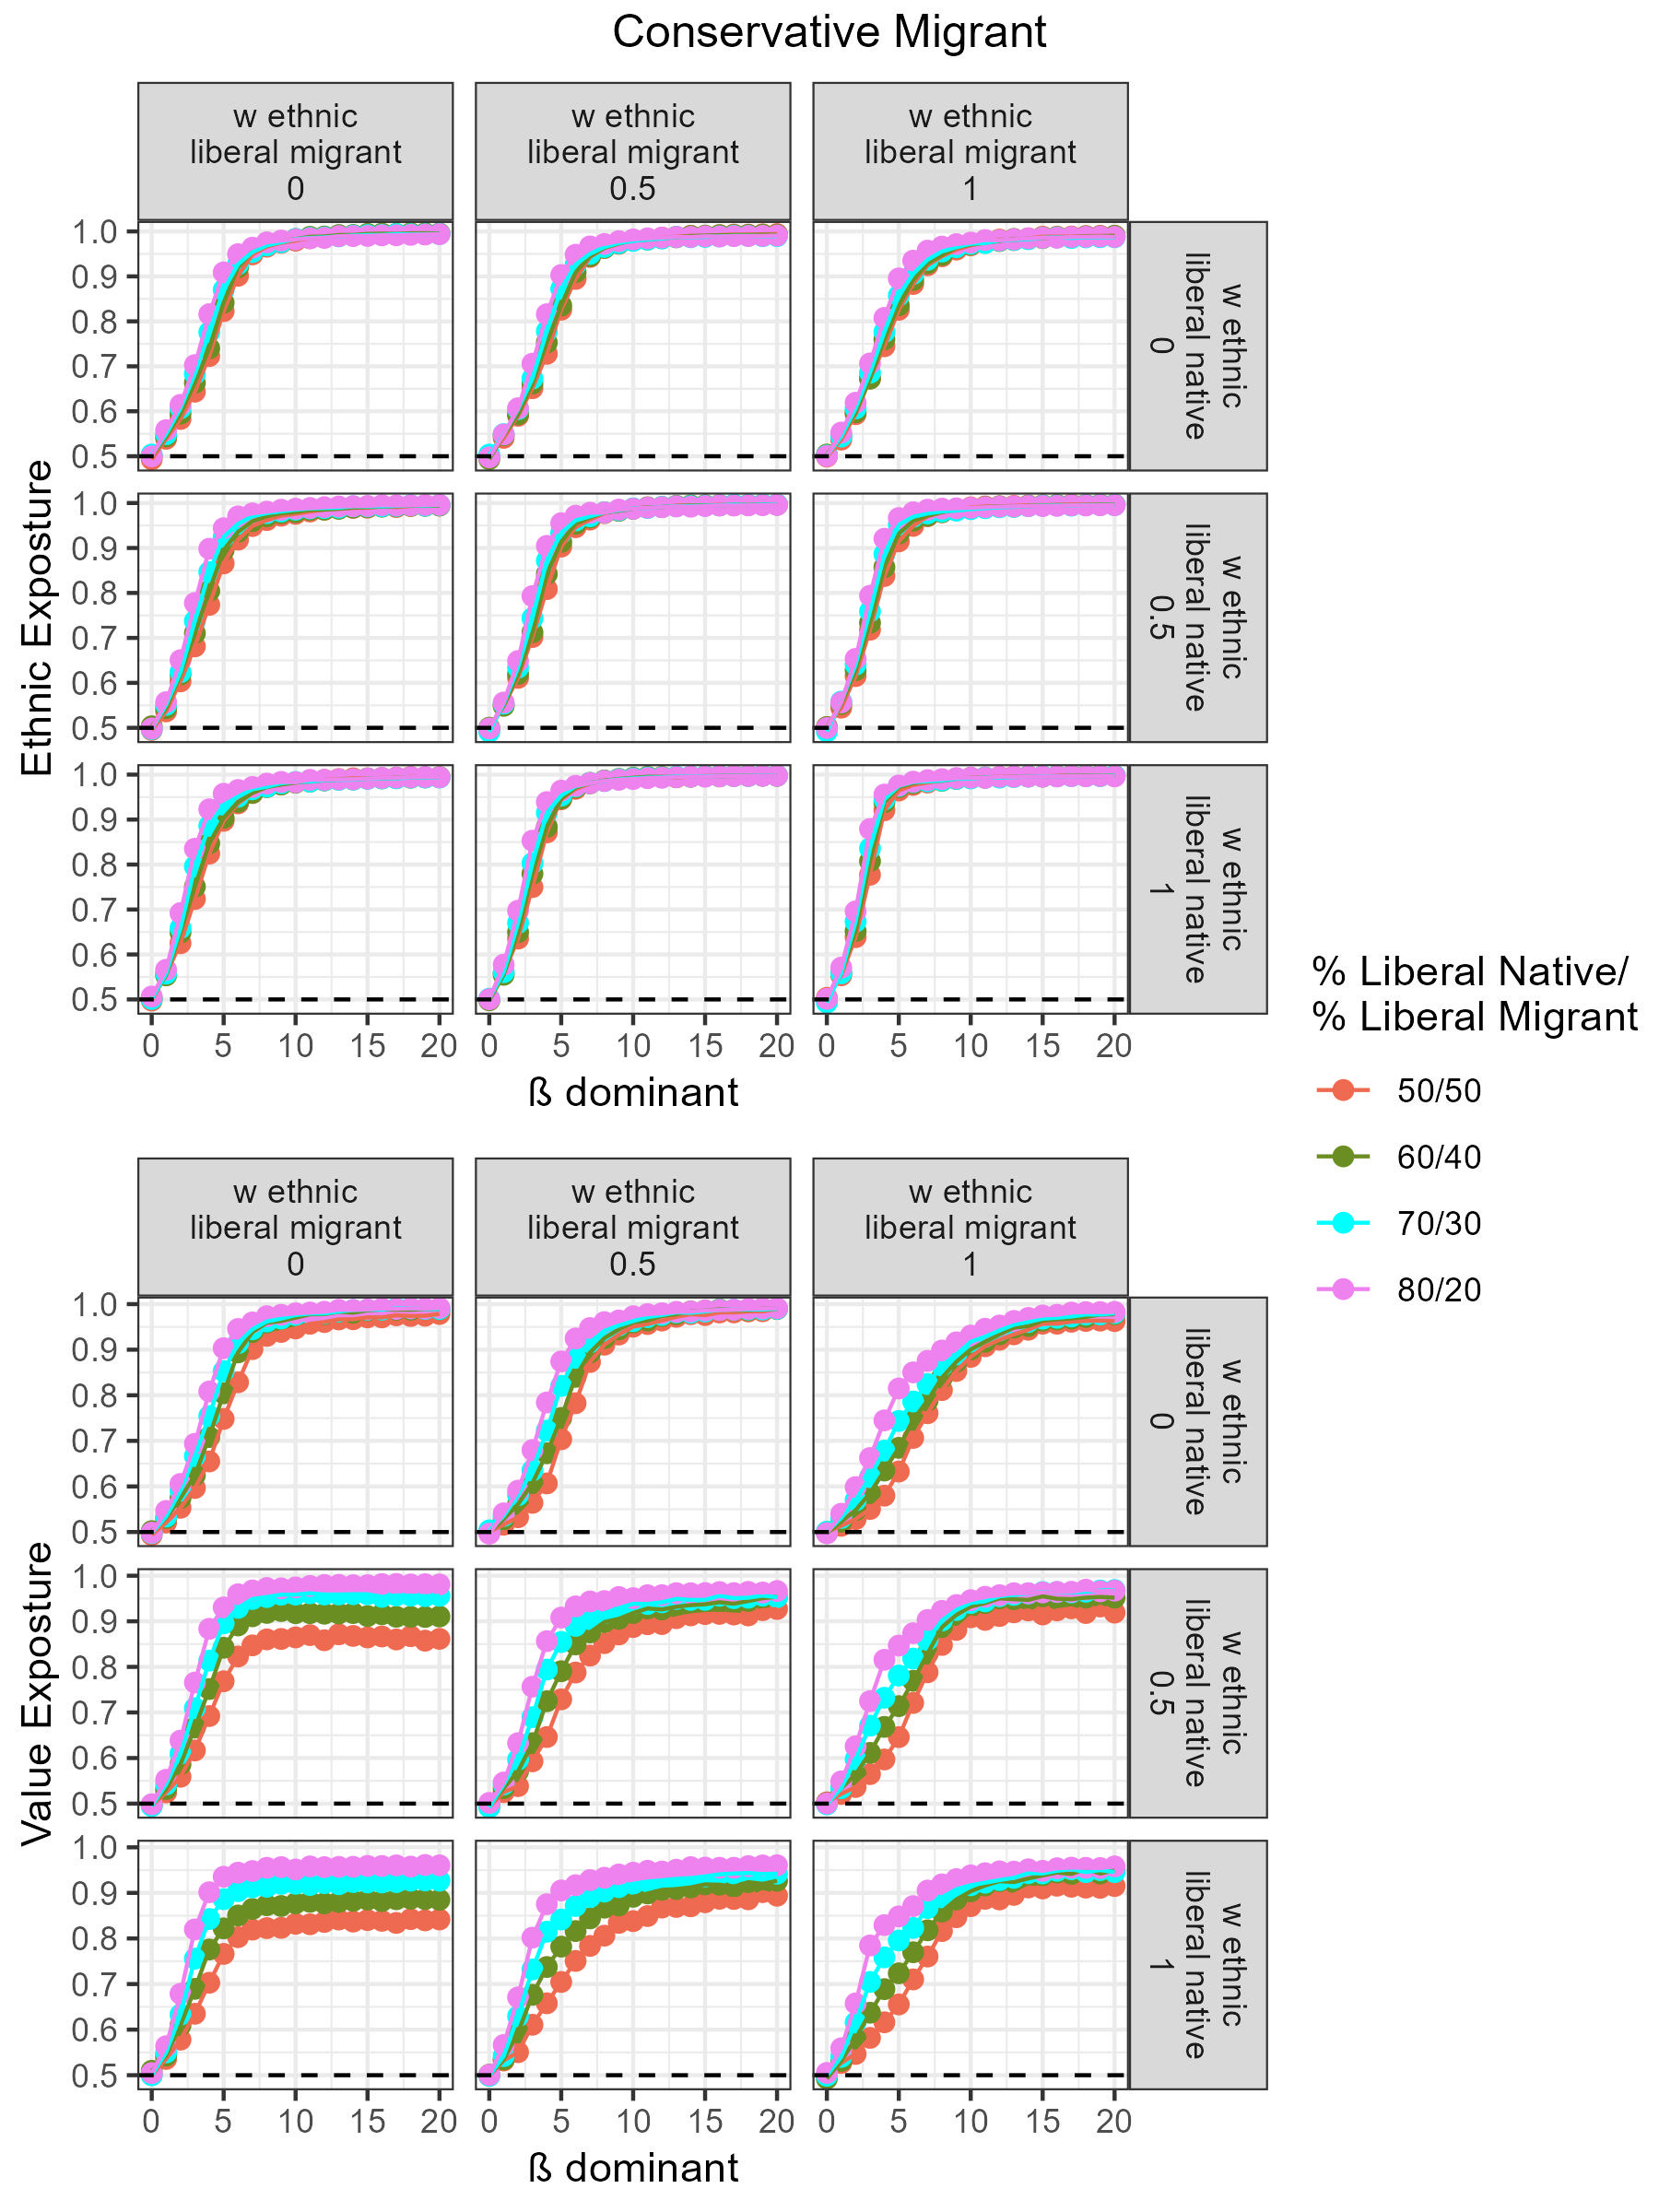
\includegraphics{images/Conservative Migrant_vlsz.jpg}
    \caption{Conservative migrant; minority/minority condition}
    \label{fig:consmig}
\end{figure}


\begin{figure}[H]
    \centering
    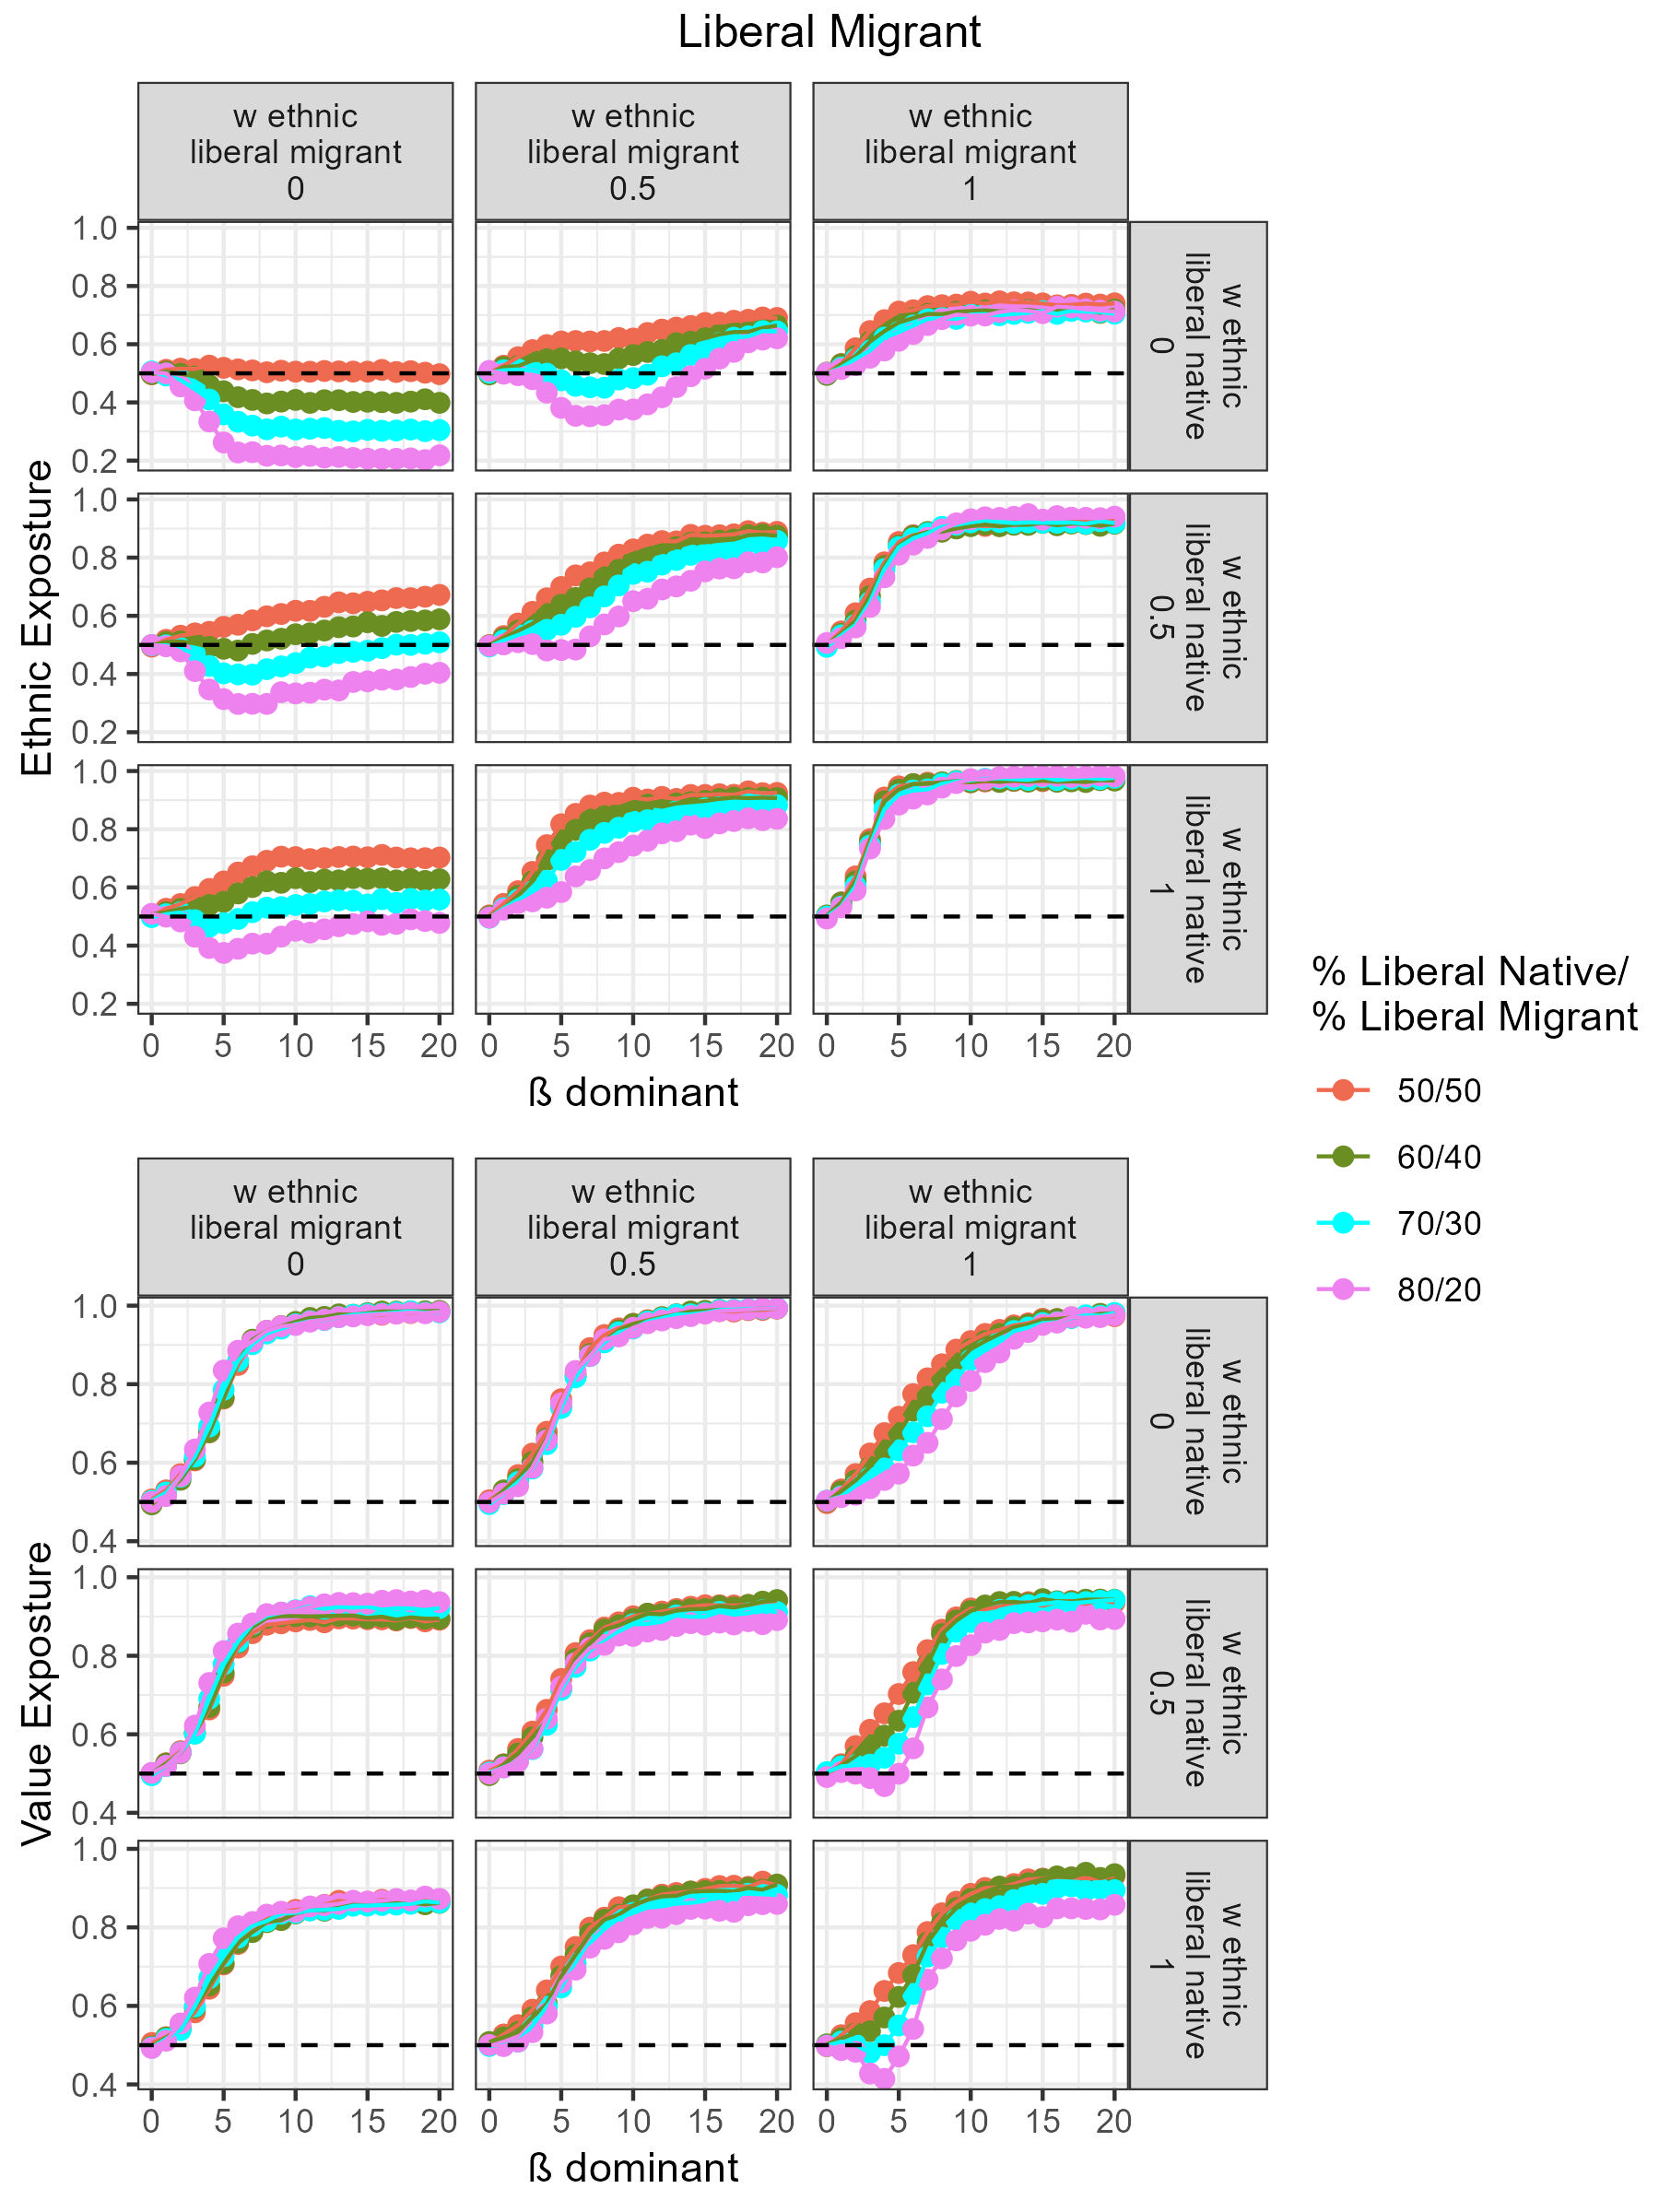
\includegraphics{images/Liberal Migrant_vlsz.jpg}
    \caption{Liberal migrant; minority/minority condition}
    \label{fig:libmig}
\end{figure}

\renewcommand\refname{References}
  \bibliography{references}

\end{document}
